\chapter{Incremental Reconstruction of Urban scenarios}
\label{ch:manif}

Urban reconstruction from a video captured by a surveying vehicle is a core module of automated mapping.
In this chapter we show how to build incrementally a manifold mesh from a monocular video by carving a 3D Delaunay triangulation of sparse points.
This approach is particular useful when computational power represents a limited resource and a detailed map is not the primary goal, for instance to analyze the traversability or to avoid obstacles.
We propose three enhancements of the state-of-the-art in incremental mesh reconstruction.
Instead of relying on points from SfM, we build the triangulation upon the 3D points reprojecting to image edges, named Edge-Points; these points constrain the edges of the triangulation to real-world edges.
We also propose the Inverse Cone Heuristic that preemptively avoids the creation of artifacts in the reconstructed surface; finally, we  efficient manage moving points, which are usually considered static, due to the overhead introduced by the update of their position in the triangulation.

\minitoc


\section{Rationale}
Urban 3D reconstruction represents a fundamental task of many robotics applications, e.g, city mapping \cite{pollefeys_et_al_08} or city segmentation \cite{Hane_et_al_09} from a surveying vehicle.
Most of the existing systems propose computationally expensive stereo methods that build a very detailed reconstruction by estimating dense keyframe depth maps , usually by means of GPU computing \cite{pollefeys_et_al_08,cornelis_et_al08}. 
In some robotics applications, a monocular, rough and computationally less expensive reconstruction is preferred,  for instance, let consider traversability analysis performed on embedded CPU-only system. 
However, if details and accuracy are needed, this reconstruction could also be refined by means of a Multi-View Stereo algorithm as \cite{vu_et_al_2012}.

Space carving \cite{seitz_et_al06} thus becomes an effective method to build  a large urban map quickly. 
Existing literature (see Section \ref{sec:incr}) proposes both batch \cite{Pan_et_al09} and incremental \cite{litvinov_lhuillier_13,lovi_et_al_11} space carving methods.
The former perform the reconstruction by taking into account all the viewing rays at the same time; the latter carve the space incrementally, \ie, frame-by-frame.
In our case we focus on the incremental approach.

The authors in \cite{lovi_et_al_11}  and \cite{litvinov_lhuillier_13} propose two incremental space carving algorithms based on the 3D Delaunay triangulation of sparse 3D point clouds. 
In \cite{lovi_et_al_11} the estimated surface is simply the boundary between free space and matter; on the other hand in \cite{litvinov_lhuillier_13}, and its extension \cite{litvinov_Lhiuller14}, the estimated surface is forced to be \emph{manifold}, \ie, for each vertex, the neighboring triangles are homeomorphic to a disk (see Section \ref{sec:manif_discr}). 

Several reasons lead to enforce the manifold property. First, most computer graphics algorithms need the manifold property to hold, one example is the Laplace-Beltrami operator \cite{Meyer03}.
Moreover, photometric surface refinement as in \cite{vu_et_al_2012} and \cite{delaunoy_et_al_08} usually needs surface manifoldness to properly compute the gradient flow that minimizes the photometric error. Finally, non-manifold surfaces are usually not realistic in real world environments.


\begin{figure}[tp]
\centering
\begin{tabular}{cc}
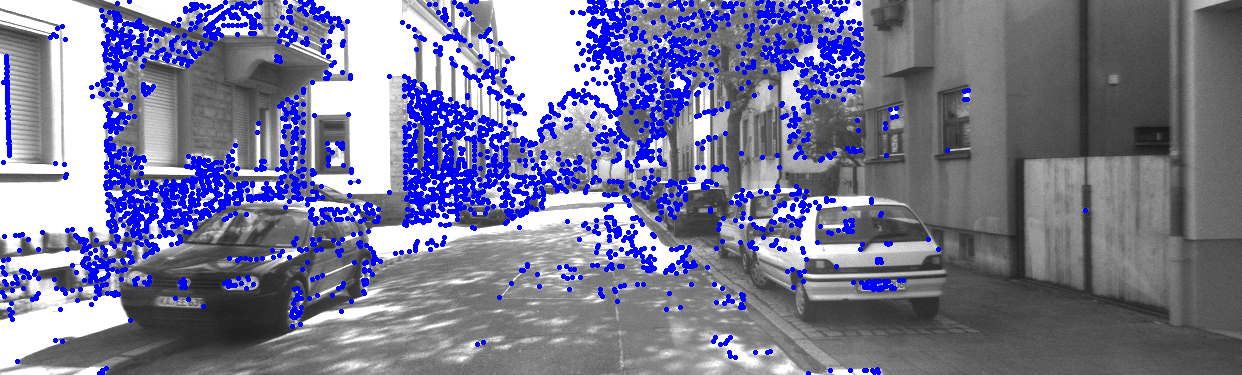
\includegraphics[width=0.92\columnwidth]{./img//harris}\\
(a)\\
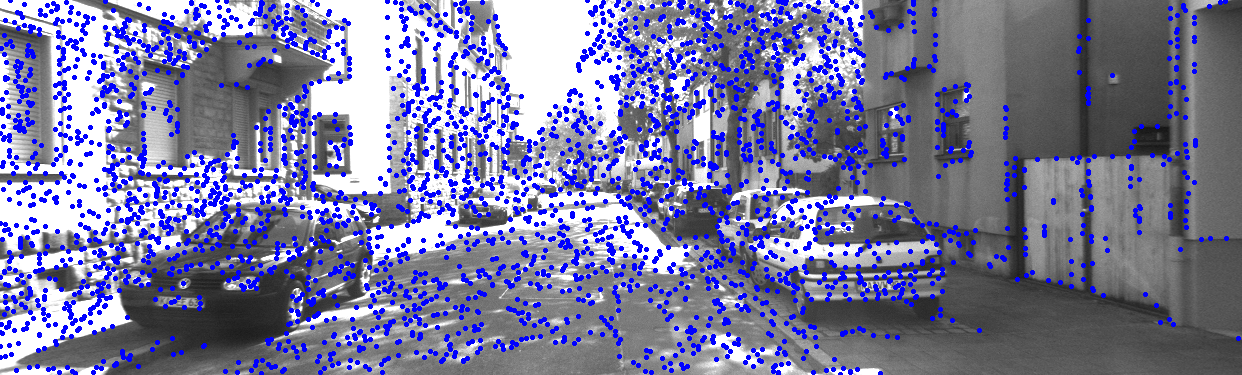
\includegraphics[width=0.92\columnwidth]{./img//edgepoints}\\
(b)\\
\end{tabular}
\caption{Different features extracted on the same image: (a) shows 3609 Harris corners, (b) shows 3595 Edge-Points.}
\label{fig:Edge-Points}
\end{figure}


\begin{figure}[tp]
\centering
\begin{tabular}{cc}
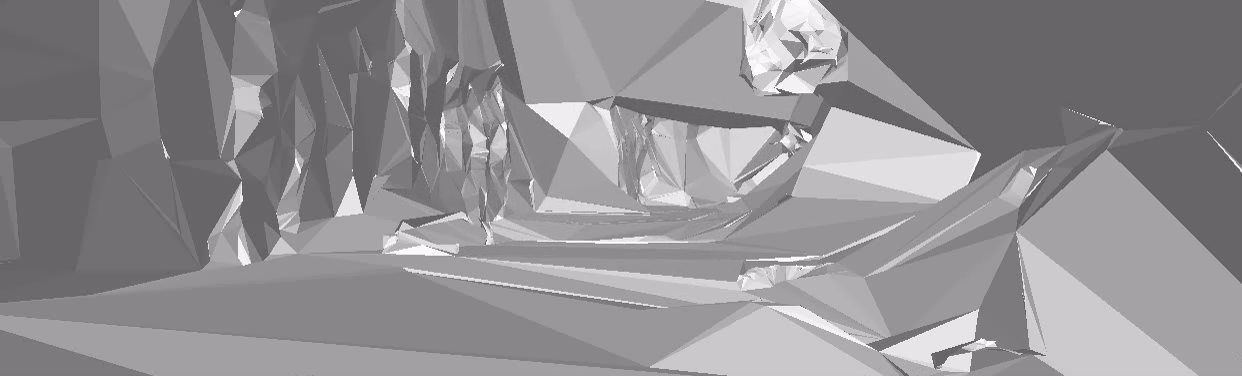
\includegraphics[width=0.92\columnwidth]{./img//reconstrHarris}\\
(a)\\
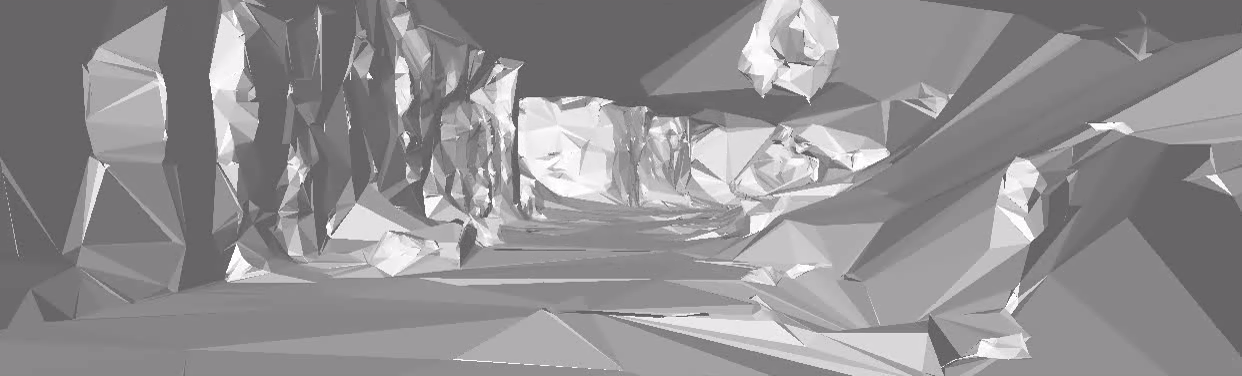
\includegraphics[width=0.92\columnwidth]{./img//reconstr}\\
(b)\\
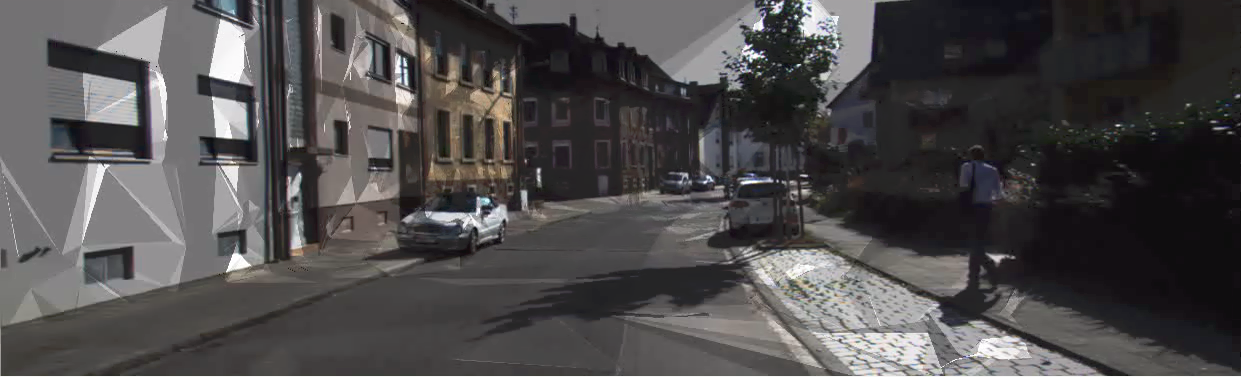
\includegraphics[width=0.92\columnwidth]{./img//reconstrTex}\\
(c)\\
\end{tabular}
\caption{Reconstructions with (a) Harris corners, (b) Edge-Points, and (c) textured reconstruction of (b).}
\label{fig:recons}
\end{figure}


Instead of reconstructing 3D points corresponding to Harris features as \cite{litvinov_lhuillier_13}, we propose to build the 3D Delaunay triangulation on the points projecting on the (Canny) edges of the images, named \emph{Edge-Points} (see Figure \ref{fig:Edge-Points}). 
The existing incremental space carving systems, \eg, \cite{litvinov_Lhiuller14, litvinov_lhuillier_13, lovi_et_al_11}, rely on sparse point cloud estimated by Structure from Motion, which discards the Edge-Points, since these are considered as instable features to track.

The main drawback of these points is the degree of freedom along the edge itself that usually causes instability in estimation and matching.
Nevertheless, several reasons supports the usaof Edge-Points.
First, urban scenarios show lot of sharp edges, therefore Edge-Points represent suitable vertexes to constrain the edges of the 3D Delaunay triangulation to real-world edges (see Figure \ref{fig:recons}). 
Then, as Figure \ref{fig:Edge-Points} shows, Edge-Points provide a better coverage of the image.
Finally, the number of Edge-Points is easier to tune with respect to the classical feature detector: by changing the downsampling rate we change proportionally the number of Edge-Points.

Other authors \cite{Rhein_et_al13, Tomono09} already took advantage of Edge-Points in their systems. Rhein \etal in \cite{Rhein_et_al13} propose a heterogeneous (corner features and Edge-Points) tracker that exploits the epipolar constraint, but, differently from us, their work is focused on the tracking stage and it aims at a sparse point cloud reconstruction.
Tomono \cite{Tomono09}  uses Edge-Points to make  the Simultaneous Localization And Mapping (SLAM) process robust in an indoor scenario that exhibits a lack of texture, but he does not reconstruct the 3D surface of the scene, moreover it uses a stereo rig that makes the estimation of the 3D point positions easier with respect to the monocular case addressed in this chapter.
The use of a monocular camera looking forward induces low parallax which makes  the estimation of the 3D point positions a non trivial task. This issue adds to the previously mentioned Edge-Points instability. 

In the following, we show that the combination of the  Kanade-Lucas-Tomasi (KLT) tracker \cite{Lucas_Kanade81}, a convenient filtering of the matches, and Gaussian-Newton optimization successfully handle Edge-Points estimation even in this complex scenario. 

Our system bootstraps from a good estimate of the camera poses, as in many urban 3D reconstruction systems \cite{ pollefeys_et_al_08,cornelis_et_al08}. 
We assume the camera pose estimation could be obtained with a Structure from Motion or SLAM technique, \eg, \cite{Snavely_et_al06},  or with an estimate obtained by fusing GPS, inertial sensors and visual odometry such as in \cite{Cucci_Matteucci14}.
This assumption enables us to estimate independently, and very efficiently, the 3D Edge-Point positions.

The removal of visual artifacts represents the second issue addressed in this chapter.
This issue was deeply studied in \cite{litvinov_Lhiuller14}, where the authors propose an ad hoc post-processing procedure that attempts to detect and remove mesh artifacts by preserving the manifold property; it runs quite fast, but its computational complexity is not negligible ($0.43$s per-frame).  
We propose a very efficient heuristic to preemptively avoid visual artifacts, which runs significantly faster than the previously mentioned procedure (around $0.001$-$0.010$s per-frame). 
We named it as Inverse Cone Heuristic since the space affected by the heuristic has the shape of a cone directed inversely with respect to camera-to-point viewing ray.

Finally, differently from Litvinov \etal \cite{litvinov_lhuillier_13}, we are able to efficiently manage the moving points inside the triangulation, such that we are able to interact with a Structure from Motion or SLAM system which incrementally updates and estimates the point positions.


%----------------------------------------------------------------------------------------------------------------------------

\section{Reconstruction through Delaunay Triangulation}
\label{sec:3D-Reconstruction}
3D reconstruction with space carving entails space discretization.
We adopt the approach of Litvinov \etal \cite{litvinov_lhuillier_13}, \ie, we choose the 3D Delaunay triangulation to partition the space into tetrahedra. 
Thanks to its self-adaptive resolution and thanks to the efficient management algorithms, 3D Delaunay triangulation has been recognized in the literature to be a convenient representation for scene reconstruction  \cite{litvinov_lhuillier_13, Pan_et_al09, labatut2007efficient, lovi_et_al_11}. 
In the following we show how we choose and we estimate the sparse point cloud upon which the triangulation is created on and how we conveniently carve the space to preemptively avoid artifacts in a  way that differs from the approach presented by Litvinov and Lhuiller in \cite{litvinov_Lhiuller14}.


%----------------------------------------------------------------------------------------------------------------------------
\subsection{3D Delaunay Triangulation of Edge-Points}
\label{subsec:pcl_estimation}
A key aspect for a 3D reconstruction pipeline, not stressed enough in the literature, is the choice of the points on which the Delaunay triangulation is built, \ie, what kind of points made up the sparse point cloud.

As most of man-made environments, urban scenarios show a lot of sharp edges, \eg, the corners of building fa\c{c}ades, the borders of windows, or the silhouettes of parked cars. Existing 3D space carving systems do not leverage on this information, but they rely only on maximally stable points.
Stable points are suitable features to track, however, a reconstruction relying on them over-simplifies the reconstructed world and it mostly fails to capture the sharp edges which do not show sharp corners too.

We propose to overcome this limitation by estimating the 3D position of Edge-Points, so to constrain the edges of the 3D triangulation to lay close to \emph{real-world} 3D edges. 
This novel triangulation generates a carved space more faithful to the real-world scene, see for instance the difference of the truck of Figure \ref{fig:reconstrEx}(a) reconstructed with the use of Harris corners in Figure \ref{fig:reconstrEx}(b), and with the Edge-Points at a low ($\frac{1}{40}$) and high ($\frac{1}{10}$) downsampling rate  in Figure \ref{fig:reconstrEx}(c) and \ref{fig:reconstrEx}(d) respectively. 

Figure \ref{fig:Edge-Points} shows that some Edge-Points have been induced by grass and shadows on the road plane. Even if this subset of features will not lay on real-world edges, their presence does not affect the quality of the reconstruction, since they lay, or are close, to the actual \emph{matter}.
Nevertheless most of these points, especially those induced by the grass, get extracted also by the Harris corner detector. 

Let stress one more time here that most of the Edge-Points lay on the real-world edges, while the Harris corners do not locate them very well.
Another important point is that it is easy to increment the number of Edge-Points used to reconstruct the environment by keeping the feature quality unchanged, while the corner-like features quality usually degrades as soon as other features are required. 
To verify this, in the experimental section we have tested our algorithm with two different downsampling rates showing that the quality of the reconstruction significantly improves as the sampling rate increases. 


\begin{figure}
\begin{center}
\begin{tabular}{cc}
\centering
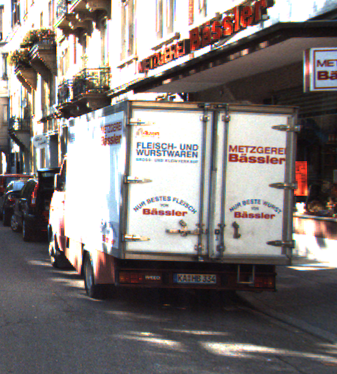
\includegraphics[width=0.33\columnwidth]{./img//imageOrig}&
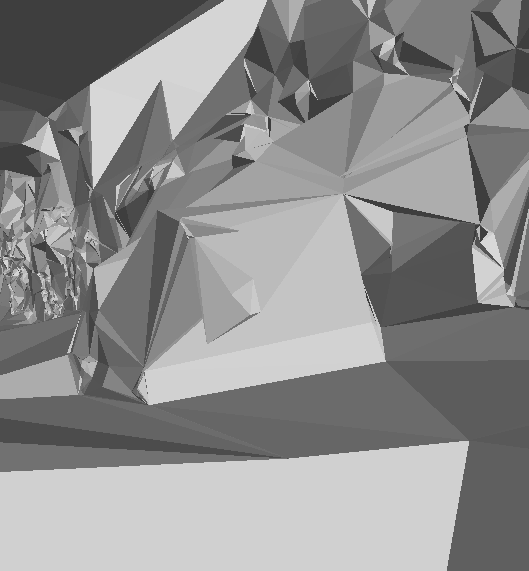
\includegraphics[width=0.33\columnwidth]{./img//notedge}\\
(a) & (b)\\
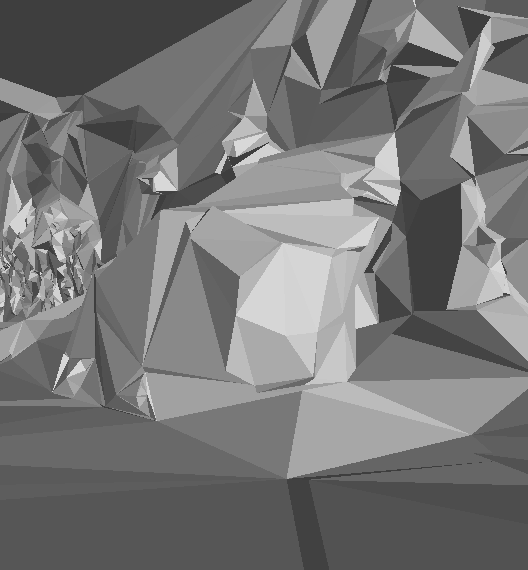
\includegraphics[width=0.33\columnwidth]{./img//edge40}&
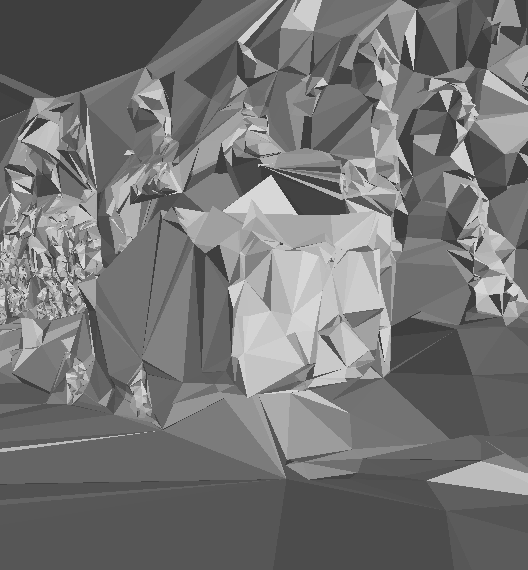
\includegraphics[width=0.33\columnwidth]{./img//edge10}\\
(c) & (d)\\
\end{tabular}
\end{center}
\caption{Three examples of reconstruction from sparse data of the light truck in (a): with Harris corners in (b), with Edge-Points with downsample rate  $\frac{1}{40}$  in (c)  and Edge-Points with  downsample rate  $\frac{1}{10}$ in (d).}
\label{fig:reconstrEx}
\end{figure}


%----------------------------------------------------------------------------------------------------------------------------


\subsubsection{Edge-Points tracking and reconstruction}
\label{subsubsec:Edge-Point-tracking}
In Figure \ref{fig:algorithm} we depict the tracking and estimation process.
For each \emph{keyframe}, \ie, one frame every $T_k$, we extract the 2D Edge-Points by (a) estimating the image edges with the Canny algorithm, and (b) downsampling those edges with step $T_{edges}$, \ie, we downsample the chains of pixels that made up the edges. 
Then we track these points in consecutive frames (both in  the keyframes and in the non-keyframes). Each \emph{track}, \ie, the sequence of point 2D positions in subsequent images, contains the \emph{measurements} of a 3D point. The value of $T_k$ depends on the camera speed; in our case of a surveying vehicle, it is fixed such that we have two keyframe per-second. 


We track the 2D Edge-Points with the KLT tracker \cite{Lucas_Kanade81} as suggested by Rhein \etal \cite{Rhein_et_al13} because it enables faster reconstruction with respect to more complex trackers which, for instance, rely on SIFT descriptor computation.
KLT tracks successfully most of the 2D Edge-Points between two consecutive frames; however, to reach good 3D point position estimates, we need to take into account errors due to the low parallax induced by the forward motion of the monocular camera and we need to filter out wrong correspondences produced by the mentioned edge instability. 


The low parallax issue affects the estimation process when the camera looks towards the moving direction. The uncertainty of the 2D point measurement on the image plane is usually assumed to be Gaussian, so the measurement uncertainty spreads in the 3D space, through the uncertainty ellipse on the image plane, as a cone whose vertex is in the camera center. 
When the parallax is low, the uncertainty cones of consecutive measurements of a 3D point are almost overlapped \cite{hazi04}. As the intersection of these uncertainty cone becomes relevant, the 3D point position estimation is no more reliable.

To ensure  an overall significant parallax and to successfully estimate the 3D points positions, we filter the tracks  both at a local and at a global level.
At a local level we filter out an Edge-Point when the displacement of its two consecutive measurements is too small, \ie, when the parallax is almost null and the uncertainty of its estimate tends to infinite. 
We experimentally set this minimum displacement to $d_{meas}^{min} = 5 \text{pixels}$ on our videos, but this parameter is related to the video frame rate and the camera focal length so it should be adapted according to the specific setup. 
Usually, as expected from the forward motion, the points filtered out lay around the center of the image, where the parallax is lower.
At a global level we discard also short tracks, \ie, those tracks containing less then $l_{track}^{min}$ measurements (we recall here that a track is the sequence of measurements of a 3D Edge-Point in subsequent images), where in our setup $l_{track}^{min} = T_K$ (recall that $T_K$ is the keyframe period). 


\begin{figure}[t]
\centering
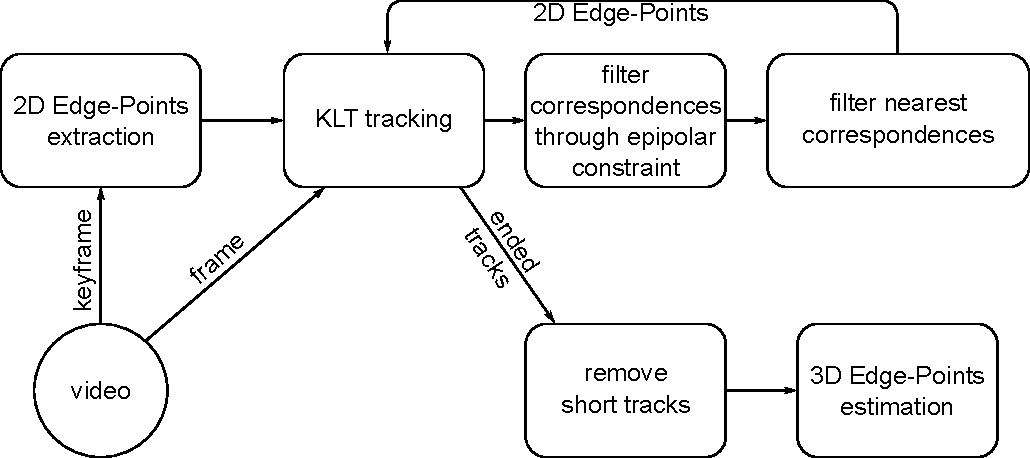
\includegraphics[width=0.8\columnwidth]{./img//EdgePoint}
\caption{Edge-Point tracking and estimation process.}
\label{fig:algorithm}
\end{figure}

To add robustness to the tracking step and manage the well-known instability  of Edge-Points  we drop the correspondences that do not satisfy the epipolar constraint. 
Let $x_{t-1}$ and $x_t$ be two corresponding points in frame $t-1$ and $t$, and $F$ the fundamental matrix between the camera at time $t-1$ and $t$, the following equation holds:
\[
 x_{t-1}^{T}Fx_t = 0 .
\]
Given $K_{t-1}$ and $K_t$ the intrinsic parameters of the two cameras, which are the same in the monocular case, and assuming the world reference frame fixed in camera $t-1$ and $P = [R_t,t_t]$ to be the pose of camera $t$, the fundamental matrix can be computed as:
\[
F = K_t^{-T}R_tK_{t-1}^T [K_{t-1}R_{t}t_t]_x
\]
where $[.]_x$ is the skew-symmetric operator \cite{hazi04}.
Given a point $x_{t-1}$ and the matrix $F$, the vector $l_{t} = Fx_{t-1}$ is the epipolar line, \ie, the locus of the points corresponding to $x_{t-1}$ in the image plane of camera $t$. 

The epipolar constraint states that, given a point $x_{t-1}$, the corresponding point $x_{t}$ lies on the epipolar line. So, given the KLT correspondence $x_{t-1}$-${x}_{t}$, we drop it if $\text{dist}_{L_2}\{Fx_{t-1}, {x}_{t}\} <\epsilon_e$, where $\epsilon_e$ is fixed to a tolerant value of $\epsilon_e = 20px$ due to the noise of the epipolar constraint estimation induced by the forward motion.
The epipolar constraint represents a necessary, but not sufficient condition. The remaining wrong correspondences will be filtered during the 3D point estimation step.

The previous filtering approach is intended to deal with almost-static scene so it filters out most of  the dynamic objects. This behavior is especially suitable for mapping purposes: in this case the map usually does not need to include dynamic object such as moving cars or pedestrians. 


Several space carving reconstruction algorithms adopt a Structure from Motion technique to estimate both  the camera pose and the 3D points position at the same time, see for instance \cite{Yu_Lhuillier12, litvinov_lhuillier_13} and \cite{lovi_et_al_11}. 
On the other hand, in urban applications, especially those involving autonomous vehicles, a very good estimate of the camera pose can be derived from sensors that are different from the camera itself (for instance with the sensor fusion technique in \cite{Cucci_Matteucci14}). 
Therefore, as in  many urban reconstruction systems (\cite{ pollefeys_et_al_08,cornelis_et_al08})  we assume the camera pose to be known, while triangulating the 3D edge-points. This assumption allows to estimate the 3D position of each 3D Edge-Point independently, \ie, in parallel.

After the tracking process, for each Edge-Point we first estimate a rough 3D position by triangulating the first and last measurements with the classic algorithm proposed by Hartley and Sturm \cite{Hartley_Sturm97}. 
We then optimize this 3D position estimate with a Gauss-Newton algorithm by minimizing the 3D reprojection error over the whole track (we fixed a number of $N_{GN} = 50$ iterations):
\begin{equation}
 e(X_{3D})^i = P^i \cdot X_{3D} - x_{meas}^i, \forall i \in \text{track}
\end{equation}
where $P^i$ is the $i$-th camera matrix, $X_{3D}$ is the 3D position of the point to be estimated, and $x_{meas}^i$ is the  measurement in the $i$-th image.
Since some wrong correspondence could exist, we drop the Edge-Points for which the mean reprojection error is higher then $\epsilon_{GN} = 2\text{px}$ at the end of optimization.





% \begin{figure}
% \centering
% \begin{tabular}{cc}
% 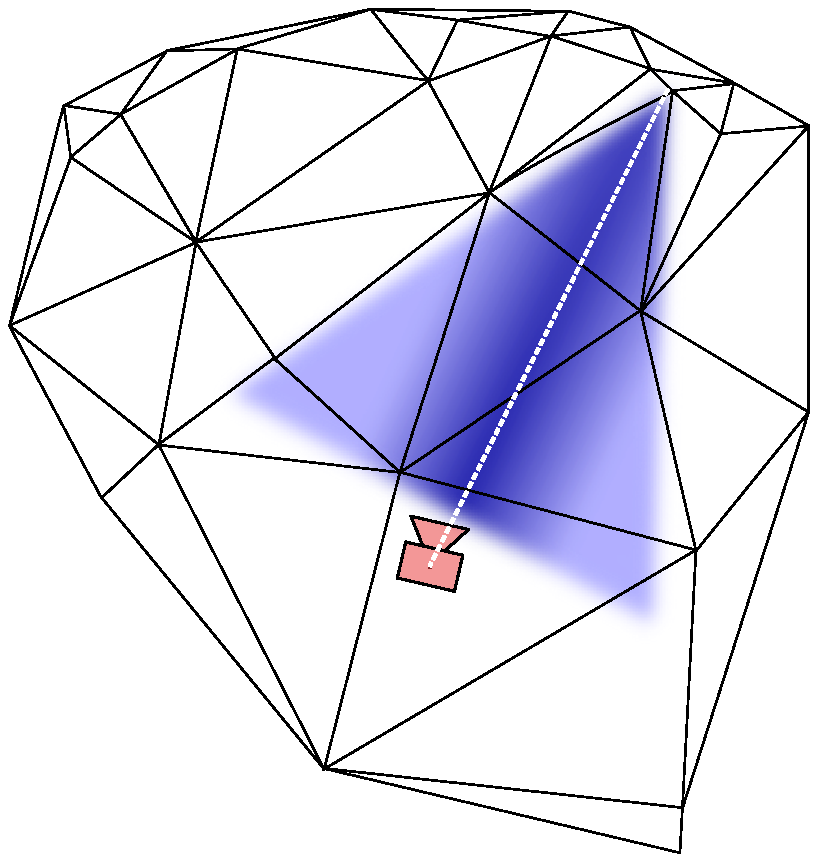
\includegraphics[width=0.45\columnwidth]{./img/conicCarvingContinue}&
% 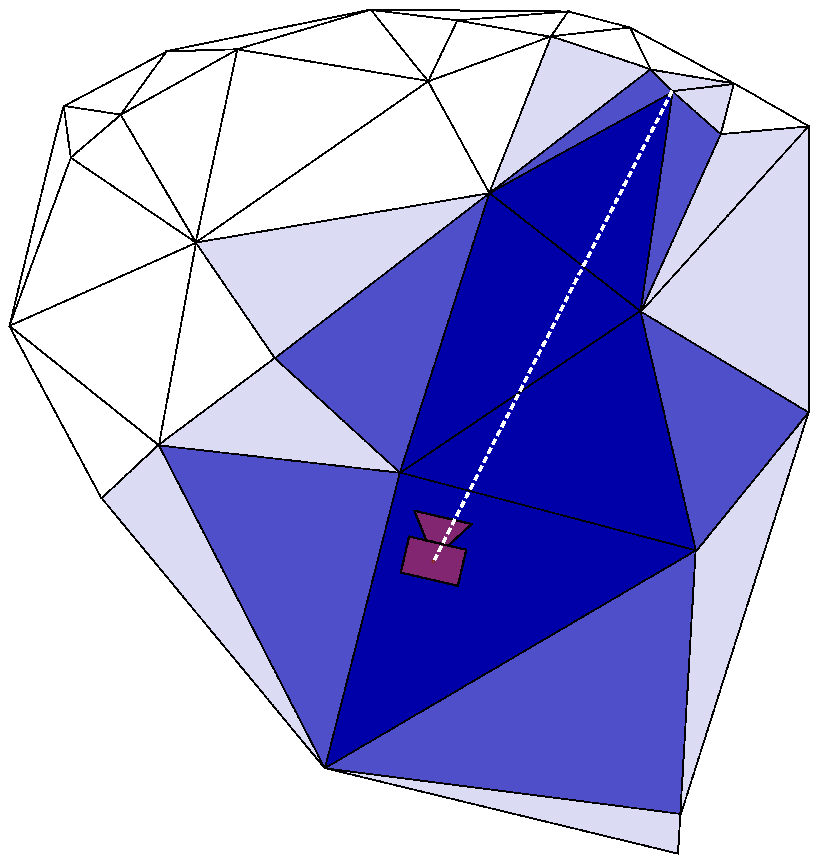
\includegraphics[width=0.45\columnwidth]{./img/conicCarvingImplemented}\\
% (a) & (b)
% \end{tabular}
% \caption{The inverse cone heuristic applied to the ray tracing step. On the left the inverse cone, and on the right our implementation in the Delaunay triangulation domain. Darker blue corresponds to higher weights.}
% \label{fig:ConicCarving}
% \end{figure}

\subsection{Inverse Cone Heuristic}
\label{sec:visualartifacts}
%----------------------------------------------------------------------------------------------------------------------------
Once the 3D Edge-Points have been estimated, we propose an enhanced version of the algorithm in \cite{litvinov_lhuillier_13}, described in Section \ref{subsec:incrementalManifold_2}, to reconstruct a manifold surface; in particular we prevent the creation of most visual artifacts affecting the state-of-the-art reconstruction.
Figure \ref{fig:artifact} shows a simple scenario where a visual artifacts is generated due to the order of tetrahedra addition to the manifold.
The algorithm bootstraps from the manifold in Figure \ref{fig:artifact}(a); then it grows the manifold by we add the triangle A (Figure \ref{fig:artifact}(b)). Afterward, C and D are free space but they are kept in the inside set, otherwise they invalidate the manifold property; this two triangles make up a visual artifact.

In our case visual artifact, which are critical for the reconstruction quality, are those containing at least one edge long enough to be considered unrealistic. 
More formally, Litvinov and Lhuiller, in \cite{litvinov_Lhiuller14}, define a \emph{critical visual artifact} as a set of tetrahedra belonging to the free space, but not included in the outside set and which contains at least one \emph{visually critical edge}, \ie, an edge $ab$ such that exists a camera center $c$ such as $\widehat{acb}>\alpha$, where $\alpha$ is a user defined parameter (in our algorithm we do not need to define this parameter).

\begin{figure}
\centering
\begin{tabular}{cc}
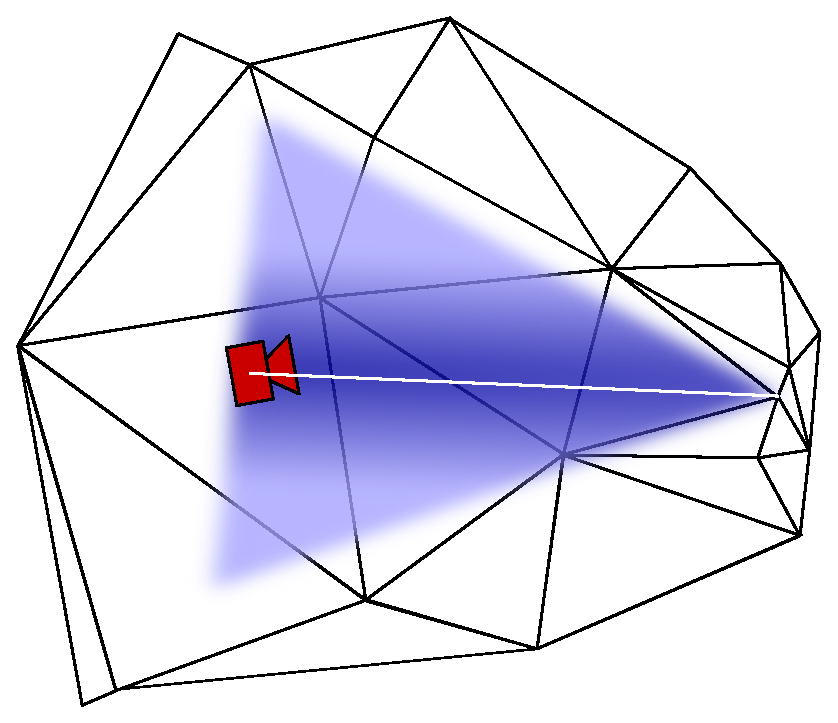
\includegraphics[width=0.35\columnwidth]{./img/ch-incr-manif/conicCarvingOKCont}&
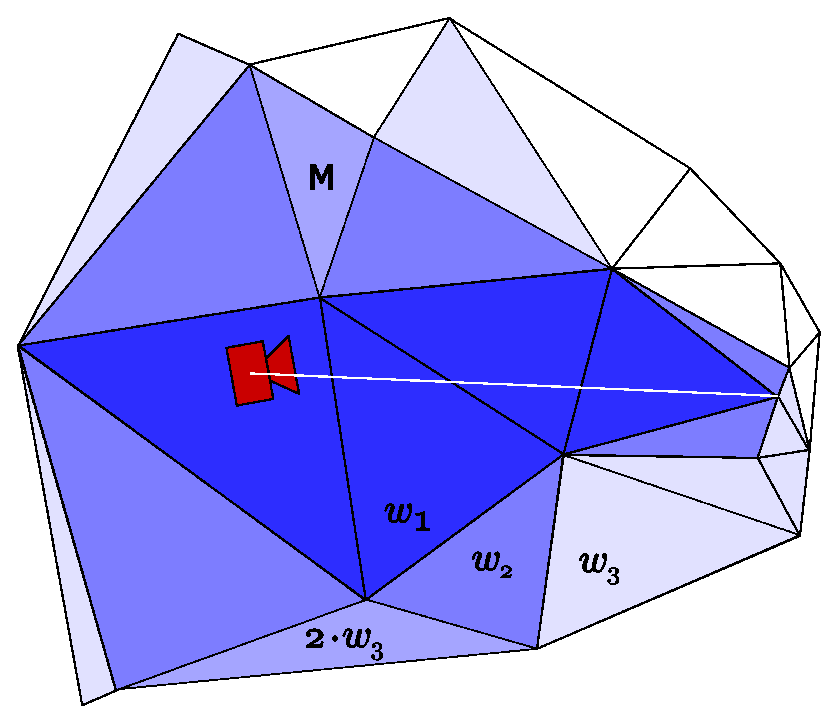
\includegraphics[width=0.35\columnwidth]{./img//conicCarvingOK}\\
(a) & (b)
\end{tabular}
\caption{The inverse cone heuristic applied to the ray tracing step. On the left the inverse cone, and on the right our implementation in the Delaunay triangulation domain. Darker blue corresponds to higher weights.}
\label{fig:ConicCarving}
\end{figure}



Litvinov and Lhuiller in \cite{litvinov_Lhiuller14}, propose a post-processing method to detect and remove critical artifacts keeping the manifold property valid.
In this paper, we propose a preemptive approach significantly different, and complementary, with respect to \cite{litvinov_Lhiuller14}. 
Our idea relies on two observations: the tetrahedra that likely turn into visually critical edges are big tetrahedra since they contains long edges, and big tetrahedra are mostly close to the camera path.





As the example of Figure \ref{fig:artifact} shows, the order of growing is a key point to avoid the creation of visual artifacts; thus,
 by modifying the ray tracing step, we aim at preemptively enforcing a carving order such that big tetrahedra near to the camera become the first to be added to the reconstructed manifold.
We replace the intersection count associated to each tetrahedron with a weight. Ideally in the continuous space, we would apply  a cone-shaped weighting heuristic, we named Inverse Cone Heuristic, which opens inversely with respect to the ray sense (see Figure \ref{fig:ConicCarving}(a)),  such that the region receiving weights increments gets smaller and smaller as the ray approaches the viewed point.
In the real discrete implementation, for each ray from the camera to the 3D point, we increment by $w_1$ the weights of the traversed tetrahedra, by $w_2$ the weights of their neighbors and by $w_3$ the weights of the neighbors of the latter tetrahedra.
Since big tetrahedra are near to the camera, this induces the cone-shaped weighting scheme as in Figure \ref{fig:ConicCarving}(b).

As Figure \ref{fig:ConicCarving}(b) shows, some ``neighbors of neighbor'' tetrahedra receive more than one increment, in particular they receive up to 4 multiple increments (one for each neighbor), but in practical cases they are usually 2 or 3.
Multiple increments let to spread the weights to tetrahedra close to the ray, without any  neighboring facet to the traversed tetrahedra, \eg,  triangle M in Figure \ref{fig:ConicCarving}(b).
To avoid high weights due to multiple increments, we tune the value of $w_3$ such that the maximum increment for neighbors of neighbor is equal to $w_2$.
For all the datasets we fixed $w_1$ to a reference value of $1.0$, then $w_2$ to a close value of $0.8$ and $w_3 = \frac{w_2}{4} = 0.2$, where 4 represents the maximum number of multiple increments received by one tetrahedra for a single ray. 


\begin{figure}
\centering
\begin{tabular}{cc}
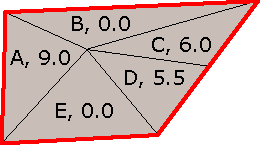
\includegraphics[width=0.35\columnwidth]{./img//artifacts01}&
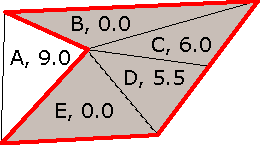
\includegraphics[width=0.35\columnwidth]{./img//artifacts02}\\
(a) & (b)
\end{tabular}
\caption{Simple scenario where a visual artifact is generated. Each triangle is labeled as ``name, weight''. The bold red line is the boundary between inside (dark triangles) and outside (white triangles) sets. Bootstrapping from (a), the triangle A is added to the manifold in (b), then neither C or D can be added anymore without invalidating the manifold property.}
\label{fig:artifact}
\end{figure}

After the ray tracing step, the region growing and shrinking procedures follows the ordering induced by the computed weights, but, to avoid carving the actual matter, one tetrahedron is added, or subtracted, to the manifold only if is traversed by at least one camera-to-point ray.




%----------------------------------------------------------------------------------------------------------------------------
\section{Reconstructing a manifold with moving points}
\label{sec:3D-Reconstruction_2}

The main limitation of the above approach is that we insert a point into the Delaunay triangulation only when its position is definitive, so, with the previous algorithm we cannot move the point position anymore even in the case we are able to refine their estimate. 

The very common approach to deal with a point moving in the triangulation, is to remove it and add it back in the new position \cite{cgal} (Figure \ref{fig:moving_ch5}). 
When we remove a point (\eg, the point A in Figure \ref{fig:moving_ch5}(a)) and we want to keep the Delaunay property, we have to remove all the tetrahedra incident to that point (light red triangles in Figure \ref{fig:moving_ch5}(b)); then, we add a new set of tetrahedra to triangulate the resulting hole (dark green triangles in \ref{fig:moving_ch5}(c)).
When we add a new point into the triangulation  (the point B in Figure \ref{fig:moving_ch5}(d)), a set of tetrahedra would conflict with it, \ie, the Delaunay property is broken (light red triangles in Figure \ref{fig:moving_ch5}(d)); so, we remove this set of tetrahedra  (red triangles in Figure \ref{fig:moving_ch5}(e)) and we add a new connected set that re-triangulate the hole (dark green triangles in Figure \ref{fig:moving_ch5}(f)).
Whenever a set of tetrahedra is replaced, we have to transfer the information about the visibility (matter or free space) of the removed tetrahedra to the new one. 
In addition to this, for each ray incident to the moved point we need to update the visibility of the tetrahedra crossed by the ray itself.
For these reasons the update of the point position is computational demanding.

\begin{figure}[t]
\centering
\begin{tabular}{ccc}
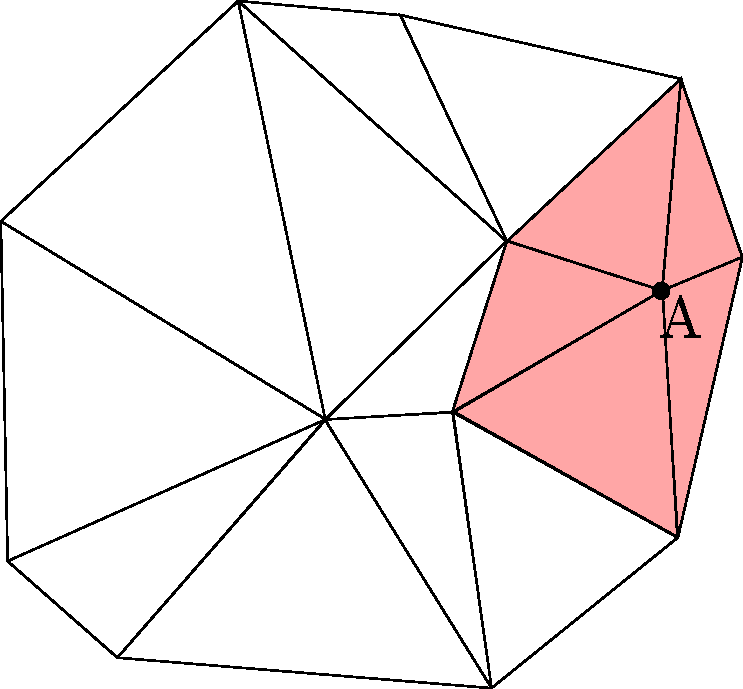
\includegraphics[width=0.28\columnwidth]{./img//delaunayExampleMoving01}&
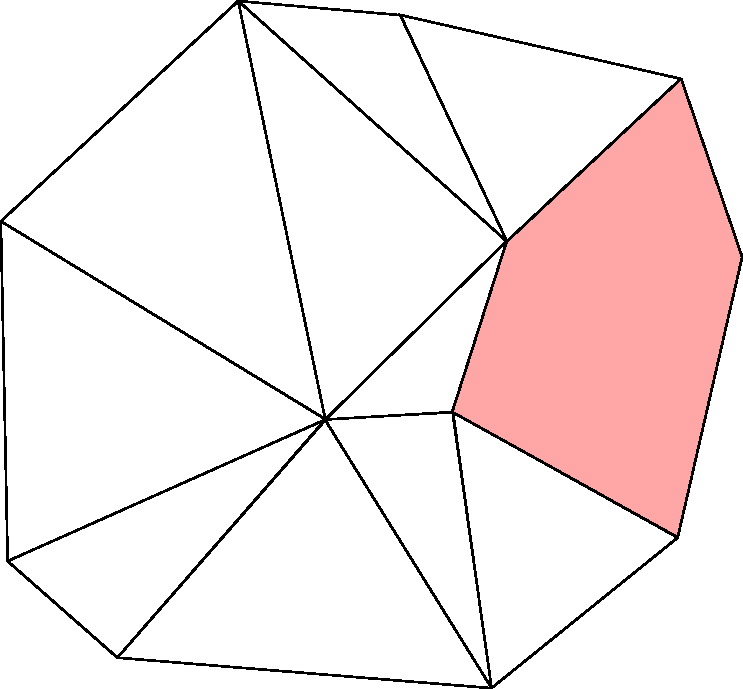
\includegraphics[width=0.28\columnwidth]{./img//delaunayExampleMoving02}&
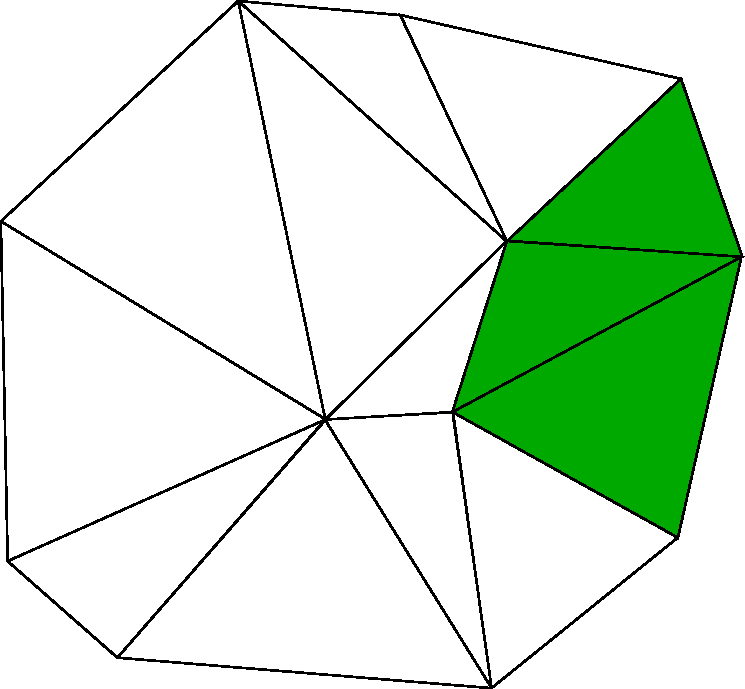
\includegraphics[width=0.28\columnwidth]{./img//delaunayExampleMoving03}\\
(a)&(b)&(c)\\
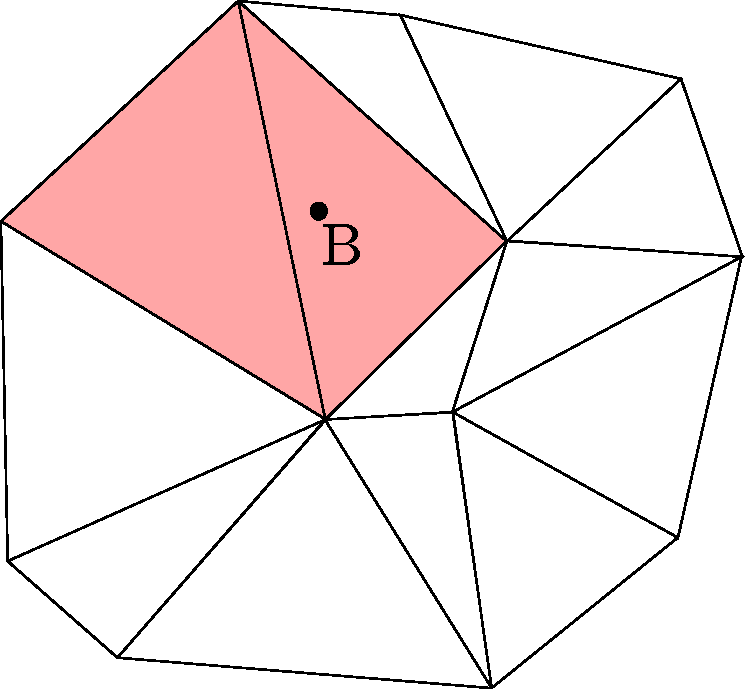
\includegraphics[width=0.28\columnwidth]{./img//delaunayExampleMoving04}&
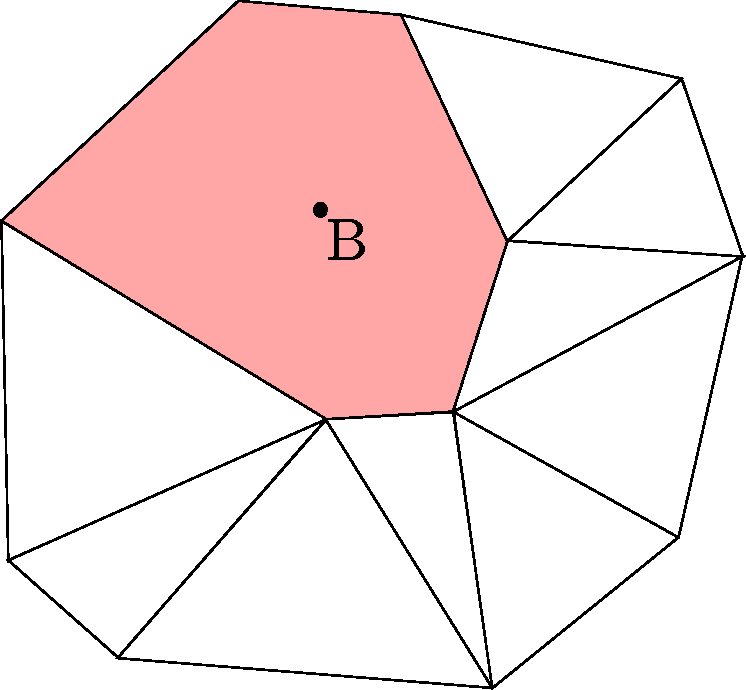
\includegraphics[width=0.28\columnwidth]{./img//delaunayExampleMoving05}&
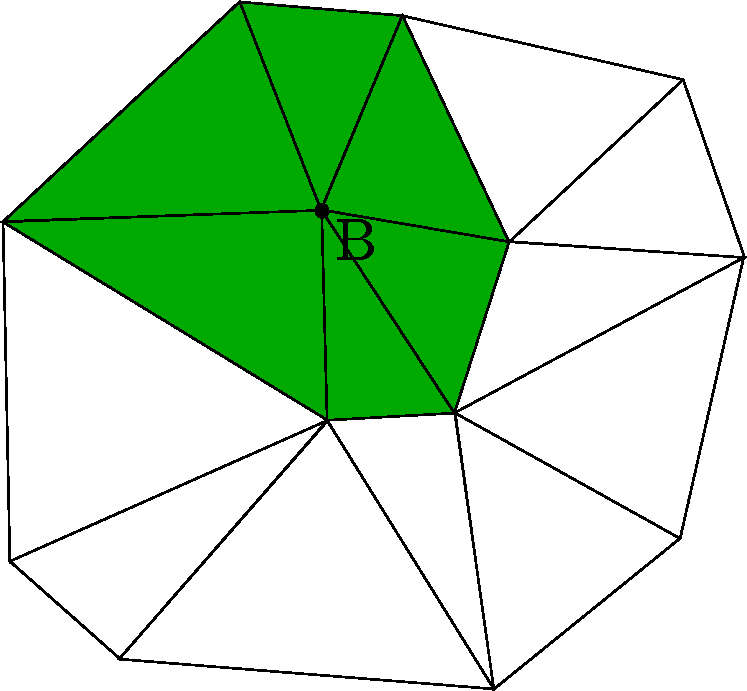
\includegraphics[width=0.28\columnwidth]{./img//delaunayExampleMoving06}\\(d)&(e)&(f)
\end{tabular}
\caption{Example of point removal in 2D case. Light red triangles depict are removed and replaced with the new dark green ones.}
\label{fig:moving_ch5}
\end{figure}

The previous algorithm, as the algorithm proposed by Litvinov and Lhuiller \cite{litvinov_lhuillier_13}, adds a point to the triangulation only when its 3D position is completely defined. 
This  restriction does not allow to refine the estimation of the position of a point 3D position after its insertion.

Only Lovi \etal \cite{lovi_et_al_11} presents an incremental Space Carving algorithm which deals with moving points, but their method does not enforce the manifold property.
In this section we verify the approach of Lovi \etal \cite{lovi_et_al_11} to be very inefficient for manifold reconstruction, and we present a different approach to deal with moving points that leads to a significantly faster computation.


\subsection{The straightforward algorithm}
\label{subsec:straightforward_way}
The simplest way to deal with moving points while reconstructing a manifold surface, is to apply a straightforward modification to the so called \emph{Refinement Event Handler} by Lovi \etal in \cite{lovi_et_al_11}.
The Refinement Event Handler algorithm assumes that, for each tetrahedron in the Delaunay triangulation a list of the intersecting viewing rays is stored. In our voting schema an intersecting ray is each ray that increase the weight of the tetrahedron. 

Let $p_{\text{old}}$ be a point that moves to position $p_{\text{new}}$, the algorithm in \cite{lovi_et_al_11} moves the point by removing point $p_{\text{old}}$ and adding $p_{\text{new}}$ as a new point, according to the classical approach of \cite{Devillers03}, then for each point they apply the following steps. 
\begin{itemize}
 \item \emph{Rays collection}: collect in a set $U$ all the rays stored into the tetrahedra incident to $p_{\text{old}}$, \ie, those affected by the $p_{\text{old}}$ removal (\eg, the light red triangle in Figure \ref{fig:moving_ch5}(a)).
 \item \emph{Vertex removal}: remove the vertex $p_{\text{old}}$ and its neighboring tetrahedra from the triangulation (Figure \ref{fig:moving_ch5}(b)); then re-triangulate the hole left by the deleted tetrahedra (Figure \ref{fig:moving_ch5}(c)).
 \item \emph{New point insertion}: insert the new point $p_{\text{new}}$ into the triangulation and add to the set $U$ all the rays stored in the conflicting tetrahedra (Figure \ref{fig:moving_ch5}(d-f)).
 \item  \emph{Rays removal}: for each tetrahedron of the entire triangulation remove the rays ending in $p_{\text{old}}$. 
 \item \emph{Ray tracing}: cast one ray for each ray in $U$.
\end{itemize}



In our case, whenever the 3D estimate of a point moves, we apply the Refinement Event Handler, before point addition and region growing, if and only if the point is inside the shrinked volume $D_{t_k}$, otherwise we do not move the point (this second case happens very rarely \cite{litvinov_lhuillier_13}), otherwise we would invalidate the manifold property.

Let consider now the computational complexity of the algorithm.
The number of rays involved in space carving algorithms is $O(F\cdot N^2)$ where $F$ and $N$ represent respectively the number of frames and the number of points in the triangulation \cite{lovi_et_al_11}, and the number of tetrahedra in a 3D triangulation grows quadratically with the number of points ($O(N^2)$). 
In Table \ref{tab:ComStraight} we reported the complexities for each of the previous stage; since our implementation exploits the CGAL \cite{cgal} 3D triangulation data structure, the complexity of a single Ray tracing, \ie, a cast of a single ray, is $O(N)$ in the general case, but we bound the size of the viewing ray, to avoid to include too far uncertain 3D points estimates, so the final complexity becomes $O(1)$  (see \cite[p.94]{yu2013automatic}).

From the analysis of the first column in the table, it is quite clear that this straightforward solution is not scalable, especially for the dependency between the number of rays and the number of processed frames. 

\begin{table}[t]
\small
\setlength{\tabcolsep}{1px}
\caption{Complexity analysis; \emph{``-''} means not existing step.}
\label{tab:ComStraight}
\centering
\begin{tabular}{lcccc}
\toprule 
Step                & straightforward     & K  & proposed     & window \\
                    & algorithm & heuristic & algorithm & heuristic \\
\midrule
Rays collection     &  $O(F\cdot N^2)$ & $O(N)$ &-&-\\
Weight collection    &-&- &  $O(N)$ & $O(N)$ \\
Vertex Removal      &  $O(N)$           & $O(N)$ &  $O(N)$           & $O(N)$ \\
New points insertion&  $O(F\cdot N^2 \cdot N)$ & $O(N)$ &  $O(F\cdot N^2 \cdot N)$ & $O(N)$ \\
Rays removal     &  $O(N^2\cdot F\cdot N^2)$ & $O(N^2)$ &-&-\\
Weight Update     &-&-&  $O(N)$ & $O(N)$ \\
Backward ray tracing &-&-    &  $O(N^2\cdot F)$ & $O(N)$ \\
Ray tracing     &  $O(N^2\cdot F)$ & $O(1)$ &  $O(N^2\cdot F)$ & $O(1)$ \\
\midrule
Overall complexity     &  $O(N^4\cdot F)$ & $O(N^2)$ &  $O(N^3\cdot F)$ & $O(N)$ \\
\end{tabular}
\end{table}


Lovi \etal \cite{lovi_et_al_11} proposed a \emph{forgetting} heuristic to limit the number of rays stored in each tetrahedron to a fixed number $K$, thus making the complexity independent from the number of the processed frames. 
However, we show in Section \ref{sec:experimental-results} that, when the points are moving,  the reconstruction is very inefficient even with this heuristic, being still quadratic in the number of frames.

\subsection{The proposed approach}
\label{subsec:efficient_way}
%----------------------------------------------------------------------------------------------------------------------------
We propose an approximation of the previous algorithm that avoids to store the list of rays inside each tetrahedron, and we just store the weight associated with it.
This allows the incremental reconstruction algorithm of Section \ref{subsec:incrementalManifold_2}, and, at the same time, we are able to bound temporal complexity.

The main difficulty in the proposed approach is updating coherently the weights whenever a point moves, \ie, when the point is removed from the triangulation and added as a new point. As soon as the point is removed from the triangulation, we perform a backward ray tracing with negative weights for each viewing camera such that the influence of the point is neglected. Then we remove the point, and we add a new vertex in the new position. Finally, we perform the ray tracing from each viewing camera to the new point.

During both point removal and addition, we have to remove a set of connected tetrahedra from the triangulation and add a new one. 
Let 
\[
 R = \{\Delta_1^R, \Delta_2^R, \dots, \Delta_{n_R}^R\}
\]
be the set of removed off tetrahedra and 
\[
A = \{\Delta_1^A, \Delta_2^A, \dots, \Delta_{n_A}^A\}
\]
the set of the new ones; their associated weights are respectively
\[
W_R = \{w_1^R, w_2^R, \dots, w_{n_R}^R\}
\] 
and 
\[
W_A = \{w_1^A, w_2^A, \dots, w_{n_A}^A\}.
\]
The weights $W_R$ are known, while $W_A$ are those to be computed for the new tetrahedra, without retracing the visibility rays related to those tetrahedra.

Different approaches are possible: 
\begin{description}
        \item[Mean value]: $w_i^A = \frac{1}{n_A}\sum_{k=1}^{n_R} w_{k}$;
        \item[Weighted mean]: let $d_{i,j}$ be the Euclidean distances between the centroids of the $i$-th tetrahedron of $A$ and the $j$-th of $R$;then $w_i^A = \frac{\sum_{k=1}^{n_R}d_{i,k}^{-1}}{\sum_{k=1}^{n_R}d_{i,k}^{-1}}$;
        \item[Minimum distance]:$w_i^A = w_{\bar{j}}^R$ such that $\bar{j} = \argmin_{j \in {1\dots n_R}}(d_{ij})$.
\end{description}


Among these, the third solution gives a non-smooth outcome and, even if this seems counter-intuitive, it results to be more suitable for our purposes. The main reason is that it preserves the discontinuity between matter and free space. For instance in Figure \ref{fig:reconstrEx_2}(a) we depict a 2D triangulation where we want to add a new point position; in Figure \ref{fig:reconstrEx_2} (b), (c) and (d) we show the results of weights update after point addition with, respectively, Mean value, Weighted Mean value and Minimum distance approaches. 
It is clear that only Figure \ref{fig:reconstrEx_2}(d) preserved the discontinuity, while in other cases it becomes hard to distinguish between matter (lower weights) and free space (higher weights). 


\begin{figure}[t]
\begin{center}
\begin{tabular}{cc}
\centering
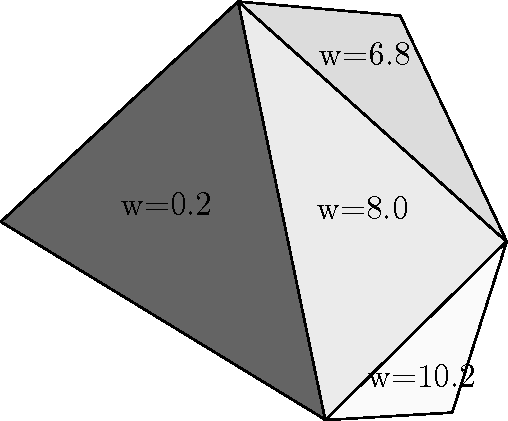
\includegraphics[width=0.42\columnwidth]{./img//mooving_orig}&
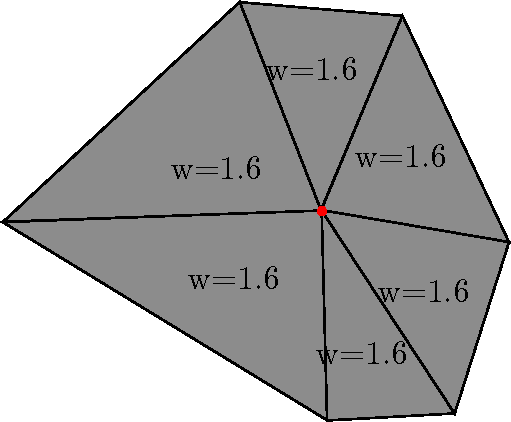
\includegraphics[width=0.42\columnwidth]{./img//mooving_avg}\\
(a) & (b) \\
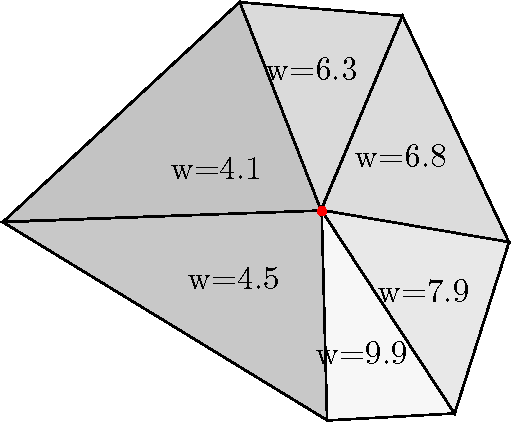
\includegraphics[width=0.42\columnwidth]{./img//mooving_weighted_avg}&
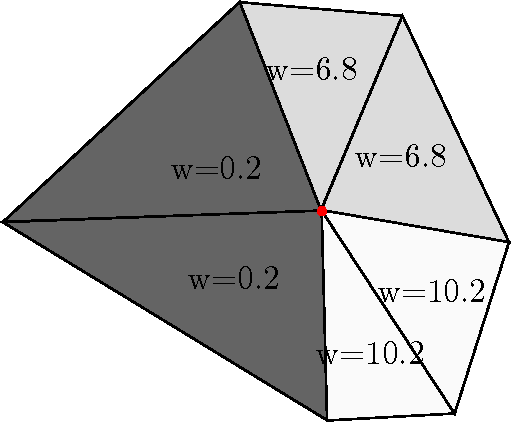
\includegraphics[width=0.42\columnwidth]{./img//mooving_min}\\ (c) & (d)\\
\end{tabular}
\end{center}
\caption{2D example of moving point addition in the new position after point removal (a brighter region corresponds to a higher weight, \ie, higher probability to be carved).}
\label{fig:reconstrEx_2}
\end{figure}

In case of very sparse data, the centroids of big tetrahedra, together with the associated visibility information, can be far from the newly added or moved points, and our update policy might result far from the ideal solution, \ie, the straightforward approach discussed in Section \ref{subsec:straightforward_way}. Our algorithm overcomes this issue thanks to the use of the (so called) Steiner points added to the triangulation before the actual reconstruction is performed; this idea was already introduced in \cite{litvinov_lhuillier_13}.
We add Steiner points to the Delaunay triangulation every 5m along each axis so that they cover all the space that can be represented. The use of Steiner points limits the creation of very big tetrahedra, the visibility information becomes always local, and the update policy avoids drifts. Indeed, experimental results show good accuracy on varied scenes, even when lack of textures induces very sparse data.


The complexity of the steps of our algorithm are reported in Table \ref{tab:ComStraight}. The main difference with respect to the straightforward algorithm is the replacement of the Rays removal with the weight update and backward tracing which are the key of the gaining in computational complexity.
The proposed algorithm is thus $O(F\cdot N^2)$, so, in principle, the dependence with $F$ still remains and results in a non scalable solution. 

\label{subsub:window}
Nevertheless, we are able to bound the complexity of our algorithm to $O(N^2)$ thanks to the following heuristic: instead of backward tracing all the rays connecting the moving point to all the viewing cameras, we consider only the most recent cameras.
In this case the complexity of the ray tracing becomes  $O(W\cdot N^2)$, where $W$ is the (constant) size  of the window (in our case $W = 15$), so the final complexity is $O(N)$.



\section{Experimental Validation}
While in \mvs many reference datasets are avaiilable, a specific monocular 3D reconstruction benchmark for urban scenarios, with accurate ground truth, does not exist; then we evaluated our contribution on four different sequences of the public available dataset \cite{Geiger_et_al12}. 
This dataset contains a Velodyne HDL-64E point cloud for each sequence which can be used as ground truth for 3D reconstruction validation.
The video stream was captured by a Point Grey Flea 2 camera, which took $1392\text{x}512$ gray scale images at $10$ fps and its view point was directed towards the direction of the vehicle motion. 
The vehicle and camera poses are estimated by a RTK-GPS and they are the initial input of our system together with the video stream.

Among all the KITTI sequences we choose the 0095 (268 frames) and 0104 (313 frames) from the raw dataset and, sequences 03 (801 frames) and 04 (271 frames) from the odometry dataset. 
They depict four different urban scenarios: the 0095 shows a narrow environment where the building fa\c{c}ades are close to the camera, the 0104 captures a wide road, while the 03 and 04 sequences provide a varied landscape mixing natural (trees and bushes) and man-made (houses, cars) features.
We run the tests on a 4 Core i7-2630QM CPU at 2.2Ghz (6M Cache) with 6GB of DDR3 SDRAM.
\subsection{Evaluation of Edge-Point Reconstruction}
\label{sec:experimental-results}
\begin{figure}[t]
  \centering
  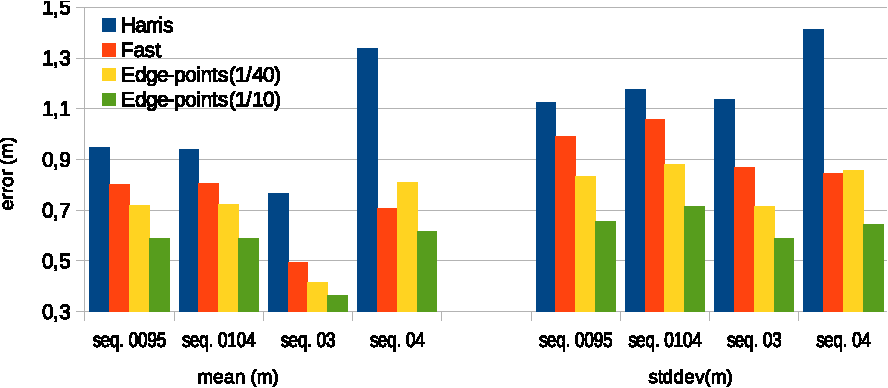
\includegraphics[width=0.98\textwidth]{./img/risultati.pdf}
  \caption{Reconstruction absolute errors of the proposed algorithm (Edge-Point) versus two classical feature based 3D reconstruction (Harris, FAST).}
   \label{tab:comp}
\end{figure}

To provide a quantitative evaluation we compared the reconstructed meshes with the very accurate point clouds measured by the Velodyne of the KITTI dataset through the CloudCompare tool \cite{cloudcompare}.
This tool was used to compute the reconstruction error, \ie, the average of the distances between each Velodyne point and the nearest mesh triangle.
Figure \ref{tab:comp} shows the comparison, on the same dataset, between the reconstruction with the proposed Edge-Points cloud and the reconstruction with the FAST and the Harris corner point clouds as in \cite{litvinov_Lhiuller14}.  
We adopted two different edge downsampling rate (low $\frac{1}{40}$ and high $\frac{1}{10}$) to verify that the accuracy gain was not a matter of number of reconstructed features, but it was due to the better choice. 
Indeed, Table \ref{tab:reconstrPt} shows that, even if the reconstructed Edge-Points with low downsampling rate are significantly less than the reconstructed points using classical features, the accuracy of the manifold estimated in the former case is always better with except to one case (sequence 04 with respect to FAST).  
The good fitting of the Edge-Points to the real 3D curves, makes the reconstructed surface to lay closer to the real one, and, in turn, this allows our Edge-Point reconstruction approach to outperform reconstructions upon non-Edge-Points.
Figure \ref{fig:distr} shows how Edge-Points have a more homogeneous distribution on the images, with respect to the other features: we subdivided the images of the sequence into a 3x5 grid and we report the percentage of extracted features for each cell.


\begin{table}[t]
  \caption{Mean number of reconstructed (and extracted) points per keyframe.}
    \label{tab:reconstrPt}
   \centering
   \begin{tabular}{p{0.2\columnwidth}cccc}
   \toprule 
                                              & 0095            & 0104        &  03         & 04   \\
   \hline   
   {Harris}                                   & 423 (2556)      & 561 (2979)  & 946 (3342)  & 692 (2036) \\
   %\hline
   {FAST}                                     & 550 (3463)      & 865 (3950)  & 1215 (4358) & 953 (2850) \\
   %\hline
  {Edge-Point (${1}/{40}$ downs.)}   & 165 (1327)      & 267 (1485)  & 404 (1650)  & 382 (1277) \\
   %\hline
   {Edge-Point (${1}/{10}$ downs.)}  & 656 (5310)      & 946 (5938)  & 1615 (6598) & 1524 (5106)  \\
    \bottomrule
  \end{tabular}
  \end{table} 

\begin{figure}[t]
  \centering
  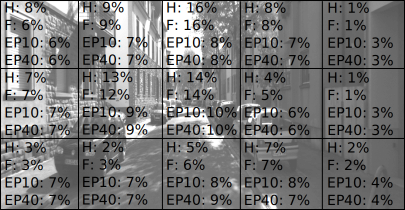
\includegraphics[width=0.9\textwidth]{././img/ch-incr-manif/distr}
  \caption{Distribution of Harris corner (H), FAST (F) and Edge-Points with downsampling $\frac{1}{10}$ (EP10) and $\frac{1}{40}$ (EP40) on the 0095 sequence.}
   \label{fig:distr}
\end{figure}


To understand how Edge-Points extraction, tracking, filtering and estimation affect the performance of our reconstruction algorithm we reported the timing in Figure \ref{tab:timing} for Edge-Points with downsampling rate $\frac{1}{10}$.
In our experiments, the tracking, filtering and estimation processing times were proportional to the number of extracted features, while the extraction depends on the selected features: the mean per-frame times are 0.0044s (Harris),  0.0010s (FAST),  0.0036 (Edge-Points with $\frac{1}{40}$ downsampling),  0.0037 (Edge-Points with $\frac{1}{10}$ downsampling). FAST is the fastest feature to extract but the impact of this step on the overall 3D estimation pipeline is almost negligible (1\% to 3\% of the pipeline).


 \begin{figure}[t]
  \centering
  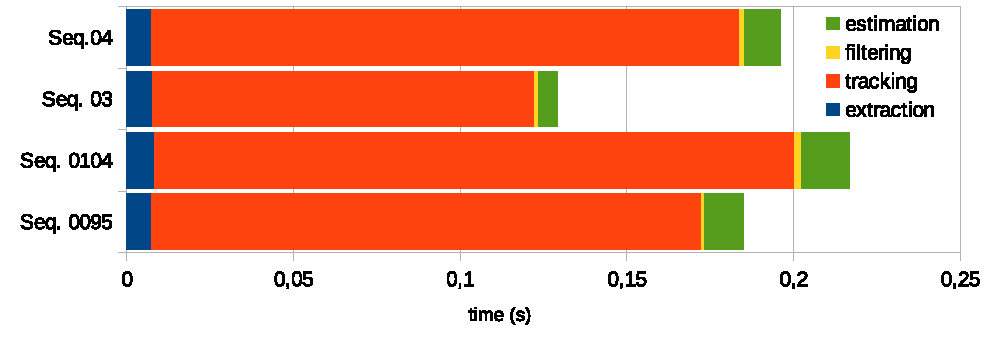
\includegraphics[width=0.98\textwidth]{././img//risultatitiming.pdf}
  \caption{Per-frame time (in seconds) of Edge-Point estimation ($\frac{1}{10}$ downsampling rate).}
   \label{tab:timing}
\end{figure}
%
  
% \begin{table}[t]
%   \caption{Mean number of reconstructed (and extracted) points per keyframe.}
%   \footnotesize
%    \label{tab:reconstrPt}
%    \centering
%    \begin{tabular}{p{0.25\columnwidth}cccc}
%    \toprule 
%                                               & 0095    & 0104    & 03      & 04   \\
%    \hline   
%    {Harris}                                   & 301     & 300 ()     & 112     & 151 \\
%    %\hline
%    {FAST}                                     & 1291    & 1322 (3950)    & 1732    & 1152 \\
%    %\hline
%   {Edge-Point (${1}/{40}$ downsample rate)}   & 447     & 521  (2979)   & 266     & 467 \\
%    %\hline
%    {Edge-Point (${1}/{10}$ downsample rate)}  & 1785    & 2077 (5938)   & 1062    &1858  \\
%     \bottomrule
%   \end{tabular}
%   \end{table} 


\subsection{Evaluation of the Inverse Cone Heuristic}
In Table \ref{tab:numArtifacts} we show the effect of the Inverse Cone Heuristic. We manually counted the visually critical artifacts in the mesh reconstructed with and without the heuristic; in parenthesis, we reported the number of artifacts affecting the camera traversability path. The heuristic diminished significantly the number of artifacts by $68$\% up to $85$\%, depending on the sequence considered. 
A fair comparison with the method in \cite{litvinov_Lhiuller14} is not possible, since their dataset and their code is not publicly available. We only point out that, in their experiments, they reported \cite{litvinov_Lhiuller14} an artifact removal rate of $35$\%.


We are also able to provide a qualitative comparison about how the Inverse Cone Heuristic affects the performance of the reconstruction. The method in \cite{litvinov_Lhiuller14} takes $0.43$s per frame on a Xeon W3530 at 2.8Ghz (8M Cache), whose performances are very similar to our machine.  The two datasets are different, but depict a similar urban scenario, and our approach (Table \ref{tab:inverseTiming}) runs one to two order of magnitude faster, thanks to the CGAL \cite{cgal} triangulation data structure which enable very efficient access to  tetrahedra neighboring the ones traversed by the camera-to-point viewing rays. 
Figure \ref{fig:exampleArt} shows a mesh without and with the inverse cone heuristic; the big artifact occluding the camera trajectory in (a) disappears in (b).
 


\begin{figure}
\centering
\begin{tabular}{c}
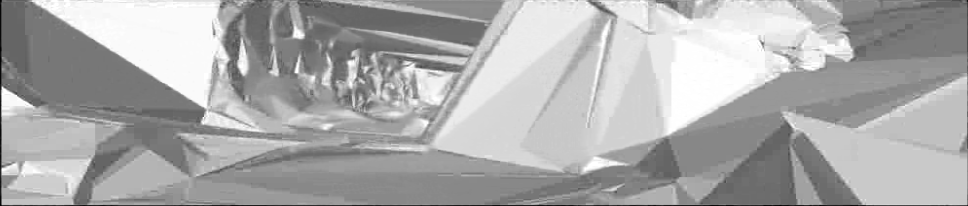
\includegraphics[width=0.92\columnwidth]{./img//inverseConeWithout}\\
(a)\\
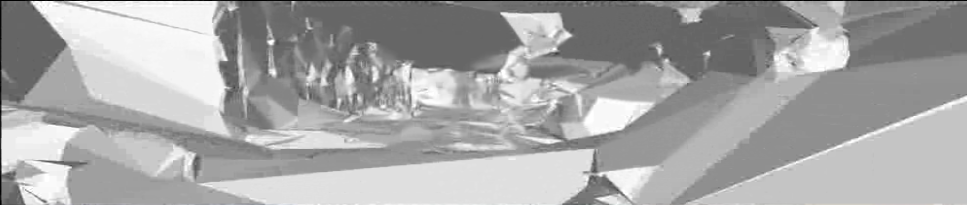
\includegraphics[width=0.92\columnwidth]{./img//inverseConeWith}\\
(b) 
\end{tabular}
\caption{Example of preemptive artifact removal: (a) without  and (b) with the Inverse Cone Heuristic.}
\label{fig:exampleArt}
\end{figure}

% Finally, we are able to conclude that the Inverse Cone Heuristic is surely effective, moreover it is possible to apply it complementary to the algorithm presented in \cite{litvinov_Lhiuller14}, since it has a really low impact on the performances. 


  

\begin{table}[t]
  \caption{Number of artifacts w/o and w/ the Inverse Cone Heuristic. In parenthesis number of artifacts affecting the camera traversability path.}
   \label{tab:numArtifacts}
   \centering
   \begin{tabular}{p{0.25\columnwidth}cccc}
   \toprule 
                               & 0095  & 0104& 03 & 04   \\
   \hline
%    {w/o ICH }                 & 21&21& 40& 22\\
%    w/  ICH                    & 4&3& 12& 7\\
%    \% removed                 & 80&85& 70& 68\\
   w/o ICH                 & 21 (4) &21(2)& 40(15)& 22(7)\\
   w/  ICH                    & 4(0) &3(1)& 12(3)& 7(1)\\
 \% removed                 & 80(100) &85(50)& 70(80)& 68(85)\\
    \bottomrule
  \end{tabular}
  \end{table}
  



\begin{table}[t]
  \caption{Per-frame time (in seconds) of the Inverse Cone Heuristic (ICH) for preemptive artifacts removal.}
   \label{tab:inverseTiming}
   \centering
   \begin{tabular}{cccc}
   \toprule  
     0095  & 0104&03 & 04     \\
   \hline
     0.002 & 0.003& 0.010 & 0.001  \\
    \bottomrule
  \end{tabular}
  \end{table} 



 % $03:801frame(154kf) 04:271(48kf) 0095:268(48kf) 0104:313(56kf)


% \begin{figure}[t]
% \centering
% \begin{tabular}{cc}
% 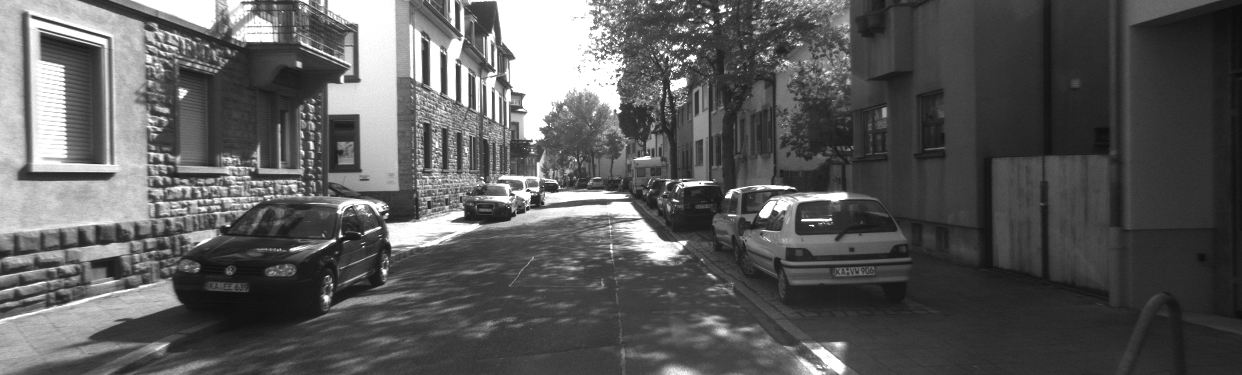
\includegraphics[width = 0.49\textwidth, height= 0.18\columnwidth]{./img//0095example}&
% 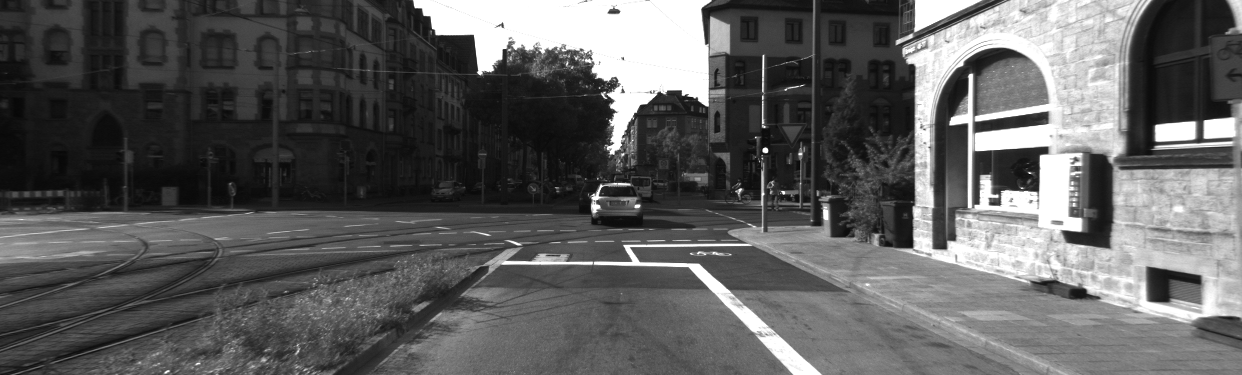
\includegraphics[width = 0.49\textwidth, height= 0.18\columnwidth]{./img//0104example}\\
% (a) Sequence 0095&
% (b) Sequence 0104\\
% 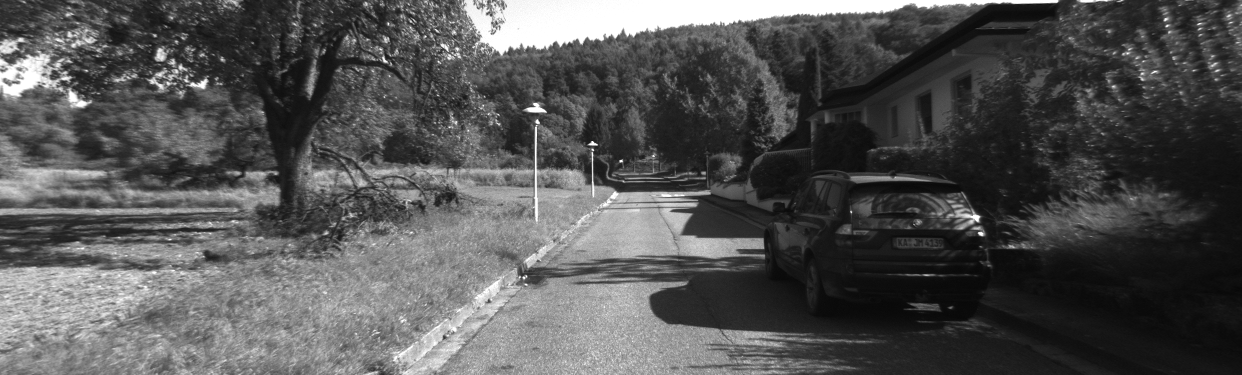
\includegraphics[width = 0.49\textwidth, height= 0.18\columnwidth]{./img//03example}&
% 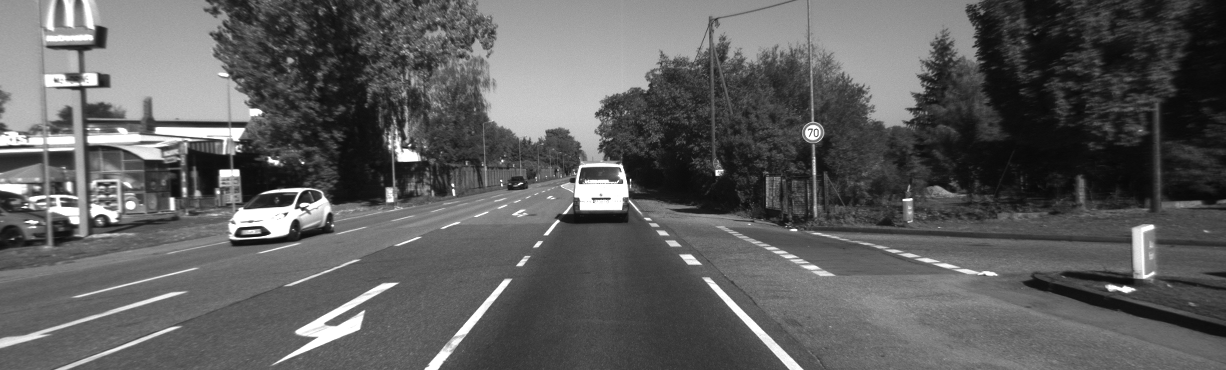
\includegraphics[width = 0.49\textwidth, height= 0.18\columnwidth]{./img//04example}\\
% (a) Sequence 03&
% (b) Sequence 04\\
% \end{tabular}
% \caption{Illustrative frames of the four sequences}
% \label{fig:exampleFr}
% \end{figure}

\subsection{Moving Points handling}

To evaluate the performances in handling the moving points in our algorithm, we compared the efficiency and the accuracy of the Lovi's approach against our three different updating policy.
As explained previously, no manifold incremental reconstruction approach deals with moving points, so a fair comparison results to be between the straightforward approach of Lovi, applied to manifold reconstruction (Section \ref{subsec:straightforward_way}) and our updating policies. In Figure \ref{fig:exampleFr} we show an example of the reconstruction results before and after the red points have been moved in the Delaunay triangulation.

Figure \ref{tab:results} shows the results of the comparison where we applied the window heuristic (Section \ref{subsub:window}) to all the algorithms. In the case of Lovi's algorithm we applied the forgetting heuristic with $K=5$ and $K=1$, where $K$ is the number of viewing rays stored for each tetrahedron.
Figure  \ref{tab:results}(a) shows that the accuracy of the proposed approach, \ie, moving point management through minimum distance weight updates, is comparable with respect to Lovi's proposal outcomes, where the algorithm with $K=5$ stores more information, so it performs better.
We compared our approach with respect to Lovi's method instead of the other incremental reconstruction algorithm presented in \cite{litvinov_lhuillier_13}; the reasons are twofold. 
In \cite{litvinov_lhuillier_13} Litvinov and Lhuiller does not deal with moving points, which is the main point addressed in this chapter. Moreover, Litvinov and Lhuiller point out in \cite{litvinov_Lhiuller14} that the ideal solution for a manifold reconstruction algorithm is represented by the manifold including as much as free space tetrahedra as possible. Since the solution provided by Lovi \etal coincides with the (non-manifold) mesh containing all the free space tetrahedra, a reconstruction accuracy similar to Lovi's suggests that the reconstruction is near to the ideal solution. In some cases our algorithm reaches even better accuracy, this is due to the smoothing effect induced by our heuristic.


Figure \ref{tab:results}(a) shows that the Minimum Distance always outperforms the other two updating schema as expected (see the Section \ref{subsec:efficient_way}).
In Figure \ref{tab:results}(b) we report the time performance of the algorithms.
Let $T_{\text{mov}}$ and $T_{\text{non-mov}}$ be the overall processing time with and without moving points, and $N_{\text{mov}}$ be the number of the total points moves, \eg, if one point moves three times, $N_{\text{mov}}=3$.
The overhead introduced in the whole reconstruction process for each move of each point has been computed as $\frac{T_{\text{mov}} - T_{\text{non-mov}}}{N_{\text{mov}}}$.
The performance of the different update schema we presented in Section \ref{subsec:efficient_way} is very similar since the steps involved are basically the same: for each update on the Delaunay data structure, we iterate over the old tetrahedra to collect the weights, then we iterate over the new tetrahedra to set the new weights.

As expected by Section \ref{subsec:efficient_way}, our algorithm clearly outperforms Lovi's approach. Our updating schema is very efficient for two reasons. 
First, we only need to update locally the visibility, while Lovi's approach casts a ray for each visibility ray stored inside the tetrahedra.
Second, when we remove a point (first step of moving point management), we perform a ray tracing backward to update only the convenient tetrahedra,  instead of iterating over the whole triangulation to remove the visibility rays involving the point moved as in \cite{lovi_et_al_11}.
  
\begin{figure}[bt]
\centering
\begin{tabular}{c}
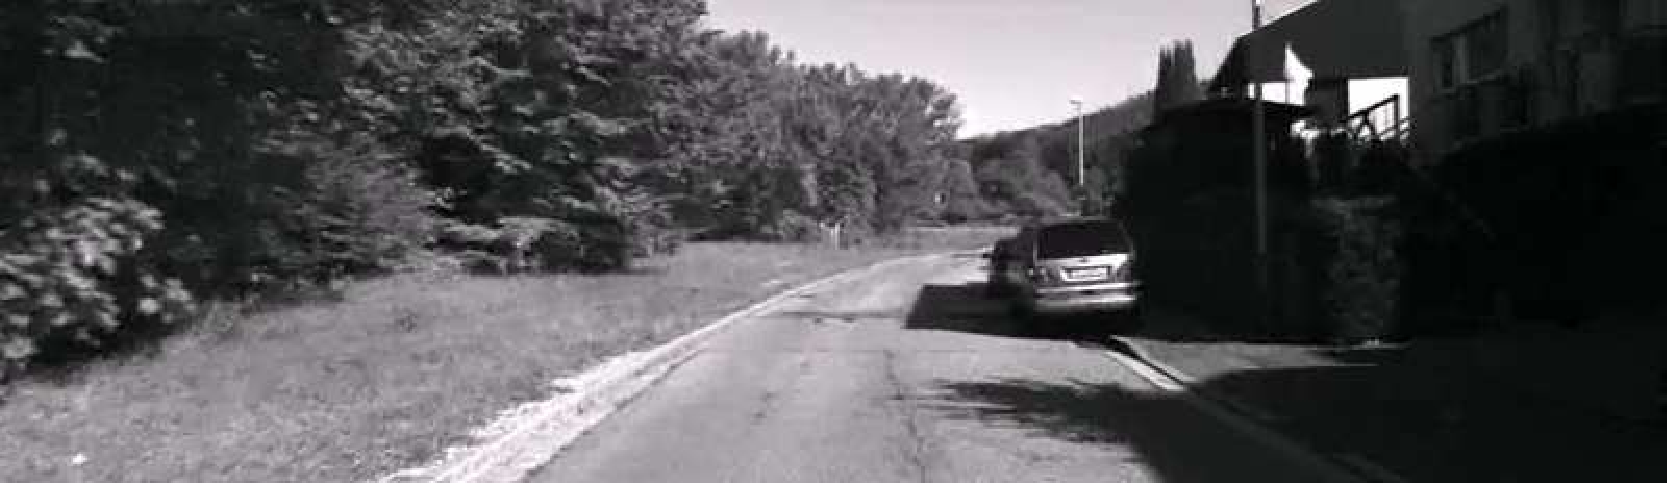
\includegraphics[width = 0.92\textwidth]{./img//ExRec_cropped}\\
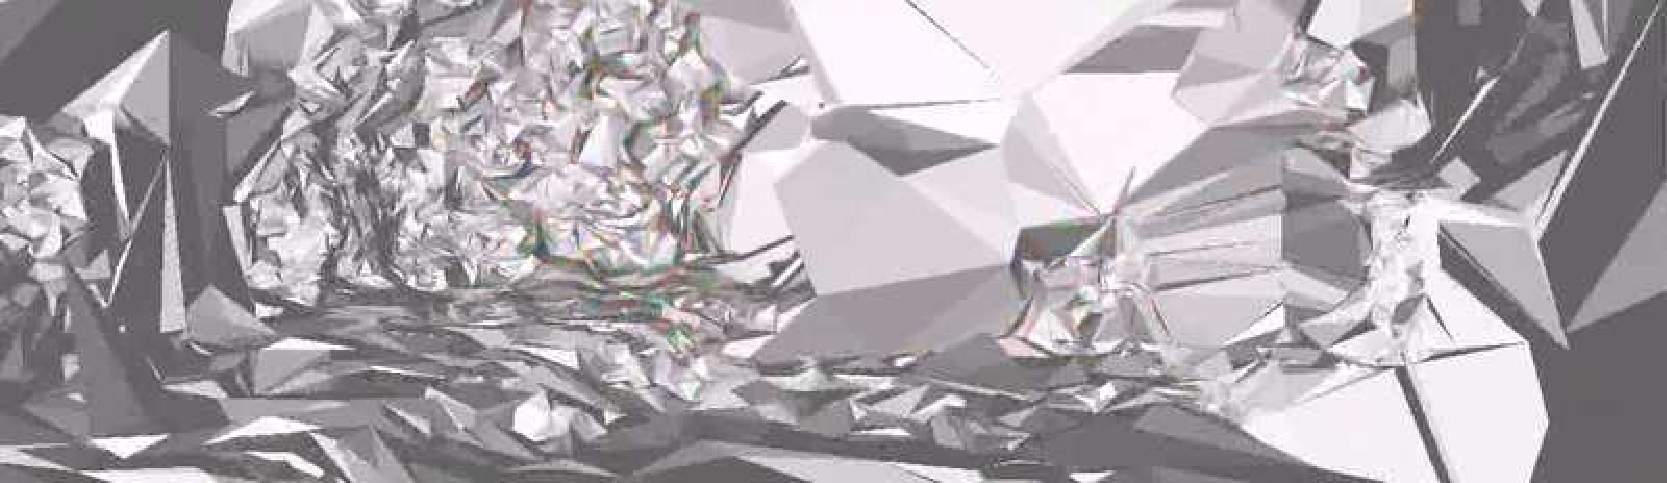
\includegraphics[width = 0.92\textwidth]{./img//ExRec01_cropped}\\
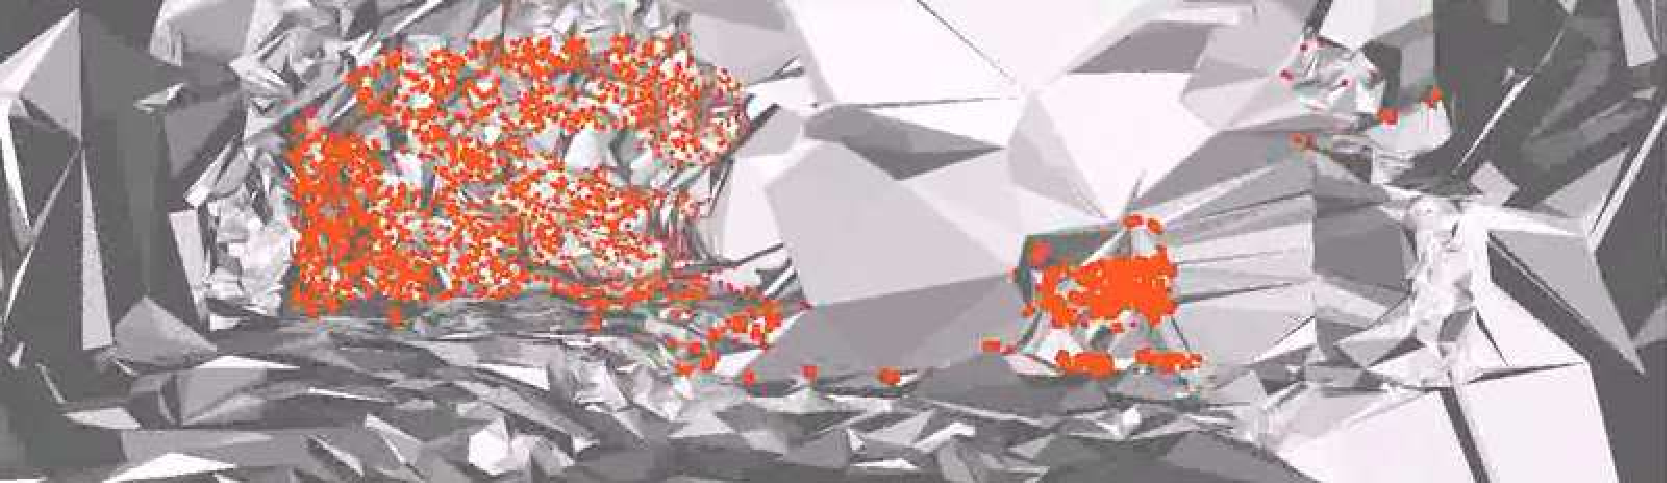
\includegraphics[width = 0.92\textwidth]{./img//ExRec02_cropped}\\
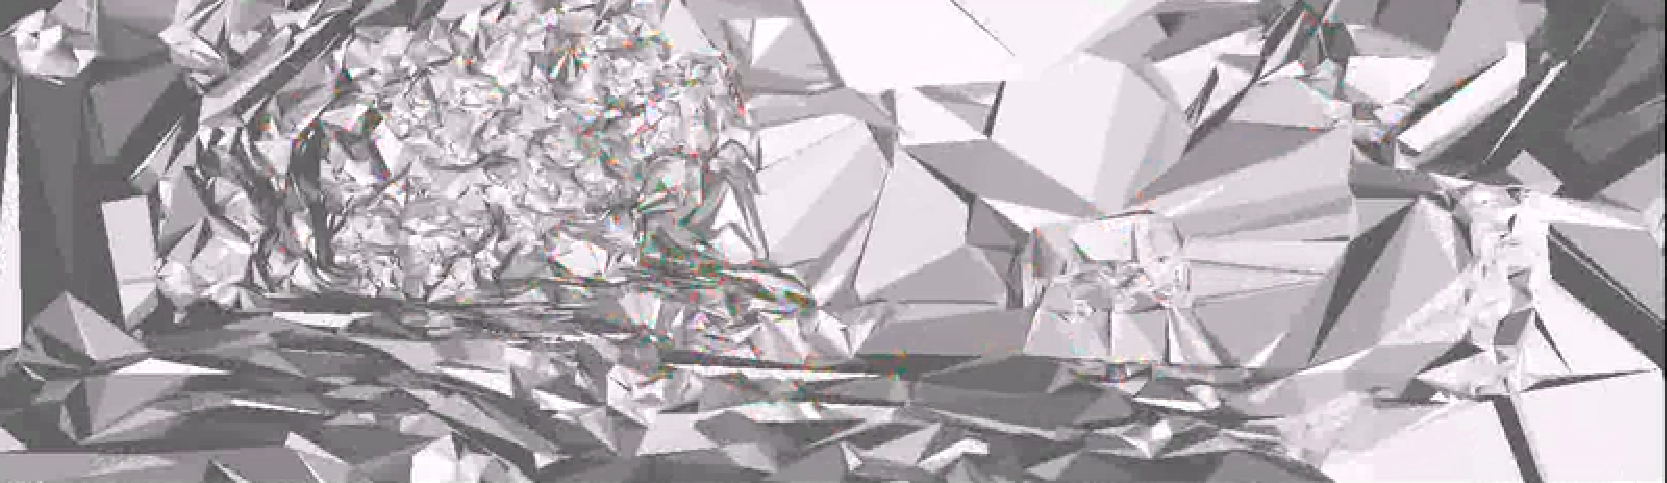
\includegraphics[width = 0.92\textwidth]{./img//ExRec05}\\
\end{tabular}
\caption{Incremental reconstruction with moving points; from up to bottom: original frame, before point positions update, points moved in the scene (red dots) and  manifold updated.}
\label{fig:exampleFr}
\end{figure}
 
\begin{figure}[t]
\centering
  \begin{tabular}{cc}
    \centering
    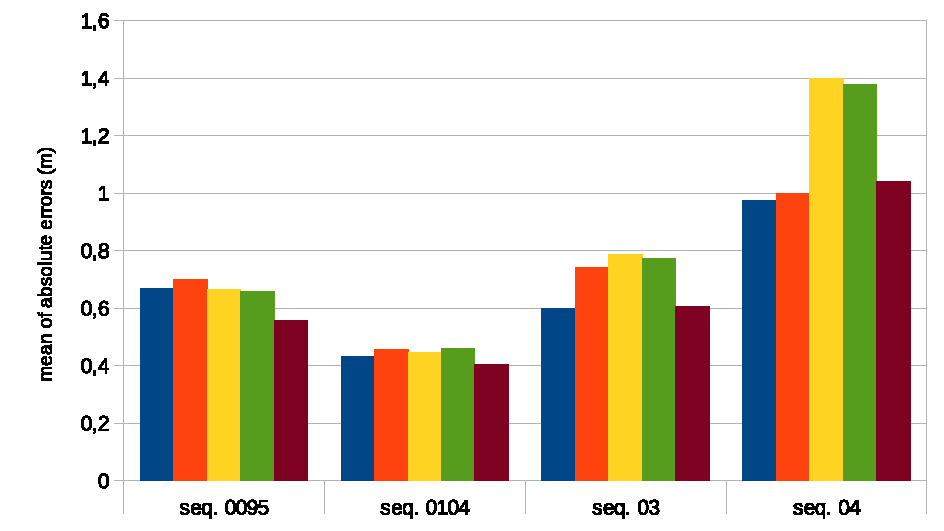
\includegraphics[width=0.72\textwidth]{./img/results.pdf}&
    \multirow{4}{*}{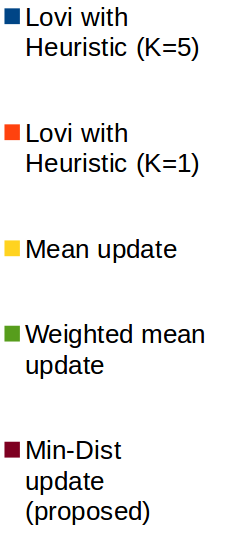
\includegraphics[width=0.2\textwidth]{./img/legenda}}\\
    (a) Absolute errors (m)\\
    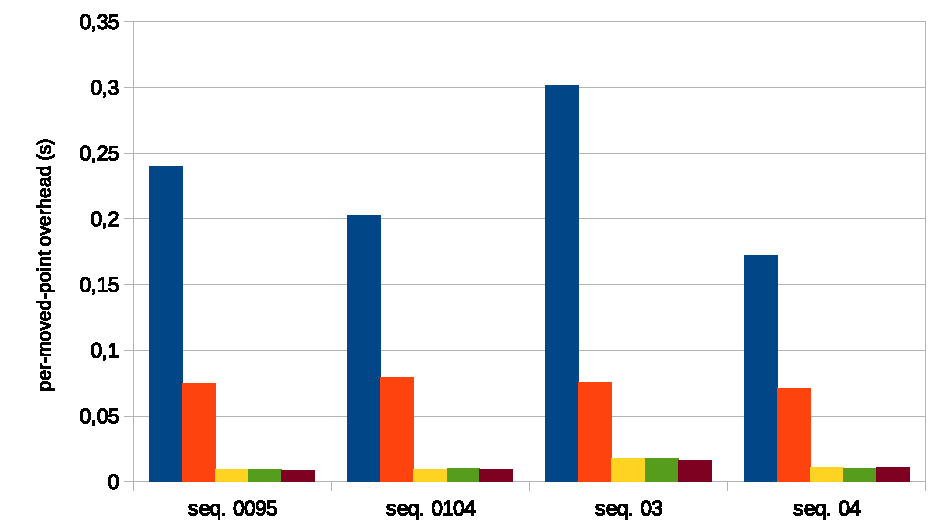
\includegraphics[width=0.72\textwidth]{./img/resultsTiming.pdf}\\
    (b) Per-point overhead (s)\\
  \end{tabular}
  \caption{Experimental evaluation of the proposed approach with respect to Lovi \etal \cite{lovi_et_al_11}.}
   \label{tab:results}
\end{figure}


%----------------------------------------------------------------------------------------------------------------------------
% \section{Summary}
% \label{sec:conclusion}
% We have shown that Edge-Points represent a very convenient choice to build a 3D Delaunay triangulation for the Space Carving reconstruction, especially in urban scenarios. We have shown how to successfully reconstruct their 3D positions by tracking their successive projections in the video images and by filtering the results of the KLT tracker with simple constraints.
% On these reconstructed points we incrementally built a 3D triangulation to reconstruct a manifold surface with a novel version of the algorithm in \cite{litvinov_lhuillier_13}
% and \cite{litvinov_Lhiuller14} improved by means of the Inverse Cone Heuristic. 
%  Moreover, we investigated the manifold reconstruction from sparse data with moving points, which resulted in a complex task. To keep the Delaunay property
% valid when a point moves inside the Delaunay triangulation, we have to remove it and add a new point in the new position. This induces the removal of a set of tetrahedra, with the associated visibility information; then, we have to add a new set of tetrahedra with coherent visibility information; finally we have to update the visibility information in all the tetrahedra affected by the point move. 
% Existing solutions successfully applied for classic space carving, resulted to be inefficient and slow when applied in the manifold reconstruction setting. We investigated different approaches to handle visibility information propagation, by updating the weight for each tetrahedron, which roughly represents the number of ray intersections, and we proposed an efficient algorithm to conveniently update it.
% The results reached by our algorithm showed that in urban scenarios the Edge-Points estimation together with Inverse Cone Heuristics enables a detailed reconstruction, which is better then those obtained by using only stable features, such as Harris or FAST corners. Moreover, we tested our update approaches to handle moving points and the proposed approaches, even if simple, clearly outperforms the existing method of Lovi \etal \cite{lovi_et_al_11}
% applied to incremental manifold reconstruction.



